%!TEX TS-program = xelatex
%!TEX root = ../../maxwell2018thesis.tex

\chapter[Snippet Lengths and Stopping Behaviour]{Snippet Lengths and\\Stopping Behaviour}\label{chap:snippets}
One of the primary components of a retrieval system that searchers interact with the~\glsfirst{acr:serp}. The presentation and design of the~\gls{acr:serp} has over the years been subject to much research. With more complex components now becoming commonplace in contemporary web search engines (such as the \emph{information card}~\citep{navalpakkam2013non_linear_serp} or \emph{social annotations}~\citep{muralidharan2012social_annotations}), much work however still remains on examining how more traditional~\gls{acr:serp} components, such as \emph{result summaries,} are designed and presented to searchers.

\begin{figure}[h]
    \centering
    \vspace{4mm}
    \resizebox{1\hsize}{!}{
    
\includegraphics{figures/ch7-serpintro.pdf}}
    \label{fig:serpintro}
    \vspace{-5mm}
\end{figure}

Result summaries (an example of which is shown above) have been traditionally viewed as the \emph{ten blue links}, each with their corresponding title and source (typically a~\gls{acr:url}) of the document. Included with these two components are the textual \emph{snippets} of \emph{keywords-in-context}, derived from the document itself. These snippets are approximately 130-150 characters (or two lines) in length~\citep{hearst2009_search}. Numerous researchers have explored result summaries in a variety of different ways, such as: examining their length~\citep{paek2004wavelens,cutrell2007eye_tracking,kaisser2008improving}; the use of thumbnails~\citep{woodruff2002summaries,teevan2009visual_snippets}; their attractiveness~\citep{clarke2007caption_features,he2012bridging}; and the generation of \emph{query-biased snippets}~\citep{tombros1998query_biased,rose2007snippet_attributes}. In essence, the length of result summaries presented to searchers has been shown to influence the point at which they stop examining the content provided in a ranked list of results. 

% The performance of searchers has broadly been evaluated in a limited fashion (for example, by examining task completion times). 

In this chapter, we are interested in examining how the length (and subsequently information content) of result summaries affects~\gls{acr:serp} interactions -- specifically examining their stopping behaviours -- and a searcher's ability to select relevant over non-relevant items. This is in tandem with an examination of different stopping strategies (outlined in Chapter~\ref{chap:strategies}), and how they adapt to increasing snippet lengths. Prior research has demonstrated that longer result summaries tend to lower completion times for informational tasks, where searchers need to find only a single relevant document~\citep{cutrell2007eye_tracking}. Does this finding however hold in an ad-hoc context, where searchers need to find \emph{several} relevant items? Furthermore, how does the length and information associated with longer result summaries affect the searcher's ability to discern the relevant from the non-relevant? We address these questions from the perspective of both:

\begin{itemize}
    \item{a \blueboxbold{user study} examining this phenomenon, as detailed in Section~\ref{chap:snippets:user}; and}
    \item{a \blueboxbold{simulated analysis}, closely examining how varying snippet lengths affects searcher performance and stopping behaviours, discussed in Section~\ref{sec:snippets:simulations}.}
\end{itemize}

The outline for both of these studies follow the general methodology, as discussed in Chapter~\ref{chap:method}. Before discussing the studies and their results, we begin this chapter with an overview of the prior work that has examined the length of result summary snippets.

\section{Background}\label{chap:snippets:background}
As previously discussed, the design and presentation of~\glsplural{acr:serp} has been examined in depth. Researchers have examined various aspects of~\glsplural{acr:serp}, and how the designs of such aspects influence the behaviour of searchers. In this section, we provide a summary of the various aspects that have been examined over time. Specifically, we consider:

\begin{itemize}
    \item{the layout and presentation of~\glsplural{acr:serp};}
    \item{the size of~\glsplural{acr:serp};}
    \item{how snippet text for result summaries is generated; and}
    \item{how much text should be presented within each result summary}.
\end{itemize}

Of the four areas of~\gls{acr:serp} research that we examine in this section, we consider the latter to be the main focus of this work. Each area is summarised below.

\subsection{SERP Layout and Presentation}
Early works regarding the presentation of result summaries examined different approaches to automatically categorising result summaries for searchers, similar to the categorisation approach employed by early search engines (as shown in Figure~\ref{fig:yahoo} on page~\pageref{fig:yahoo}). ~\cite{chen2000order_to_web} developed an experimental system that automatically categorised result summaries on-the-fly as they were generated. For a query, associated categories were then listed as verticals, with associated document titles provided underneath each category header. Traditional result summaries were then made available when hovering over a document title. Subjects of a user study found the interface easier to use than the traditional \emph{ten blue links} approach -- they were 50\% faster at finding information displayed in categories. This work was then extended by~\cite{dumais2001results_in_context}, where they explored the use of hover text to present additional details about search results based upon user interaction. Searching was also found to be slower with hover text, perhaps due to the fact that searchers were required to consider decision about when to seek additional information explicitly.

Alternatives to the traditional, linear list of result summaries have also been trialled (like grid-based layouts~\citep{resnick2001modeling, kammerer2010interface, chierichetti2011two_dimensional_presentation}). For example,~\cite{kammerer2010interface} examined differences in searcher behaviour when interacting with a standard list interface, compared against a tabular interface (title, snippet and~\gls{acr:url} stacked horizontally in three columns for each result), and a grid-based layout (result summaries placed in three columns). Those using the grid layout spent more time examining result summaries, and demonstrated promise in overcoming issues such as \emph{position bias}~\citep{craswell2008click_models}, as observed by~\cite{joachims2005click_model}.

\cite{marcos2015snippets_web_search} also performed an eye-tracking user study examining the effect of searcher behaviour while interacting with~\glsplural{acr:serp} -- and whether the \emph{richness} of result summaries provided on a~\gls{acr:serp} (i.e. result summaries enriched with metadata from corresponding pages) impacted upon the user's search experience. Enriched summaries were found to help capture a searcher's attention. Including both textual and visual representations of a document when presenting results could have a positive effect on relevance assessment and query reformulation~\citep{joho2006presentation}. Enriched summaries were also examined by~\cite{ali2009interaction_interfaces} in the context of navigational tasks. Striking a good balance between textual and visual cues (i.e. \emph{proximal cues,} as discussed in Section~\ref{sec:stopping_background:theoretical:ift:patch}) were shown to better support a searcher's tasks, and search completion time.

\subsection{Generating Snippet Text}
Searchers can be provided with an insight by result summaries as to whether a document is likely to be relevant or not~\cite{he2012bridging}. Consequently, research has been undertaken that examined different kinds of snippets, and how long a snippet should be. Work initially focused upon how these summaries should be generated~\citep{pedersen1991snippet, landauer1993enhancing, tombros1998query_biased, white2003task, leal2015query}. These early works proposed the idea of summarising documents with respect to the query (query-biased summaries), or keywords-in-context -- as opposed to simply extracting the representative or lead sentences from the document~\citep{kupiec1995tds}. Examples of both approaches are illustrated in Figure~\ref{fig:snippet_types}. Indeed,~\cite{tombros1998query_biased} showed that subjects of their study were likely to identify relevant documents more accurately when using query-biased summaries, compared to summaries that were simply generated from the first few sentences of a given document. Query-biased summaries have also been more recently shown to be preferred on mobile devices, too~\citep{spirin2016snippets}.

\begin{figure}[t!]
    \centering
    \resizebox{1\hsize}{!}{
    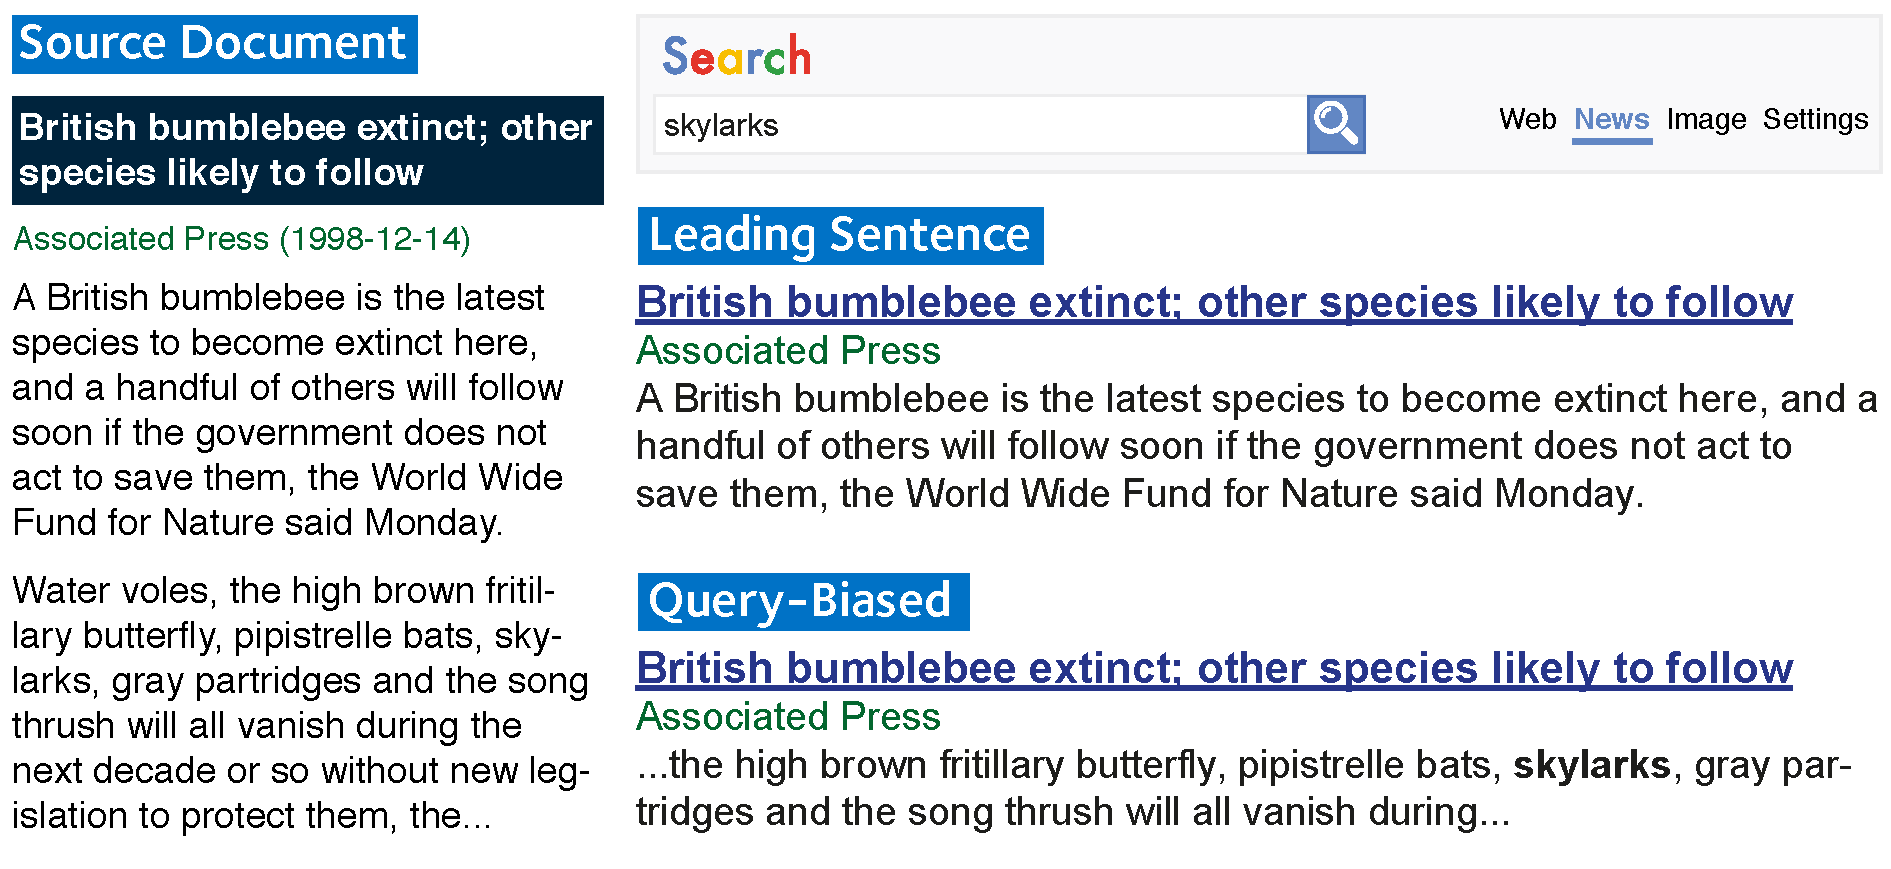
\includegraphics{figures/ch7-snippet_types.pdf}}
    \caption[Leading sentence and query-biased summary examples]{A visual example of two different types of summary, along with a portion of an example document from the~\gls{acr:trec} AQUAINT collection. Given the query \texttt{skylarks}, the \searchlogo~result summaries for both leading sentence and query-biased summaries are shown. Note the highlighting of the term \textbf{skylarks} in the query-biased summary.}
    \label{fig:snippet_types}
\end{figure}

When constructing snippets using query-biased summaries,~\cite{rose2007snippet_attributes} found that a user's perceptions of the result's quality were influences by the snippets. If snippets contained truncated sentences or many fragmented sentences (denoted as \emph{text choppiness}), searchers perceived the quality of the results more negatively, regardless of length.~\cite{kanungo2009snippet_readability} found that poor readability also impacted upon how the resultant snippets were perceived. They maintain that readability is a crucial presentation attribute that needs to be considered when generating a query-biased summary.~\cite{clarke2007caption_features} analysed thousands of pairs of snippets where result \emph{A} appeared before result \emph{B}, but result \emph{B} received more clicks than result \emph{A.} As an example, they found results with snippets which were very short (or missing entirely) had fewer query terms, were not as readable, and attracted fewer clicks. This led to the formulation of several heuristics relating to document surrogate features, designed to emphasise the relationship between the associated page and generated snippet. Heuristics included:

\begin{itemize}
    \item{ensuring that all query terms appeared in the generated snippet (where possible);}
    \item{withholding the repeating of query terms in the snippet if they were present in the page's title; and}
    \item{displaying shortened, easily readable~\glsplural{acr:url}.}
\end{itemize}

Recent work has examined the generation of snippets from more complex angles -- from manipulating underlying indexes~\citep{turpin2007fast_snippets, bast2014snippet_generation}, to language modelling~\citep{li2010snippet_extraction, he2012bridging}, as well as using a searcher's recorded history to improve the snippet generation process~\citep{ageev2013summaries, savenkov2011search}. Previous generation approaches also may not consider what parts of a document searchers actually find useful.~\cite{ageev2013summaries} incorporated into a new model post-click searcher behaviour data, such as mouse cursor movements and scrolling over documents, producing \emph{behaviour-based snippets.} Results showed a marked improvement over a strong text-based snippet generation baseline. Temporal aspects have also been considered --~\cite{svore2012temporal_snippets} conducted a user study that showed searchers preferred snippet text with \emph{trending} content in snippets when searching for trending queries, but not so for general queries.

\subsection{Results per Page}
Today, a multitude of devices are capable of accessing the~\gls{acr:www} -- along with a wide range of different screen resolutions and aspect ratios. The question of how many result summaries should be displayed per page therefore becomes hugely important, yet increasingly difficult to answer. Examining behavioural effects of mobile devices when interacting with~\glsplural{acr:serp} has attracted much research as of late (e.g.~\cite{kim2012small_vs_large, kim2014eye_tracking, kim2016pagination_versus_scrolling}), and with each device capable of displaying a different number of results \emph{above-the-fold}\footnote{Refer to Section~\ref{sec:serp:method:serp_dp} for a detailed explanation on displaying results \emph{above-the-fold.}}, recent research has shown that the number of results shown per page can influence the behaviour of searchers~\citep{joachims2005click_model, kim2014eye_tracking}. Understanding this behaviour can help guide and inform those charged with designing contemporary retrieval system user interfaces.

In a Google industry report,~\cite{linden2006} however stated that searchers desired more then 10 results per page, despite the fact that increasing the number of results displayed yielded a 20\% drop in traffic. It was hypothesised that this was due to the extra time required to dispatch the longer~\glsplural{acr:serp}. This drop however could have been attributed due to other reasons.~\cite{oulasvirta2009serp_size} discussed the \emph{paradox of choice}~\citep{schwartz2005paradox_of_choice} in the context of search, where more options (results) -- particularly if highly relevant -- will lead to poorer decisions, degrading searcher satisfaction. In terms of searcher satisfaction, it can be argued that modern search engines can therefore be a victim of their own success, leaving searchers with \emph{choice overload.}~\cite{oulasvirta2009serp_size} found that presenting searchers with a six-item result list was associated with higher degrees of searcher satisfaction, confidence with choices and perceived carefulness than a list of 24 items.

\cite{kelly2015serp_size} broadly agreed with the findings of~\cite{oulasvirta2009serp_size}. Here, the authors conducted a between-subjects study with three conditions, where subjects were assigned to one of three interfaces -- a baseline interface, showing 10 results per page (the traditional \emph{ten blue links}), and two interfaces displaying 3 and 6 results per page respectively. Their findings showed that individuals using the 3 and 6 results page page interfaces spent significantly longer examining top ranked results, and were more likely to click on higher ranked documents than those using the 10 results per page interface. Findings from this study also suggested that subjects using the interfaces showing fewer results per page found it comparatively easier to find relevant content than those using the 10 results per page interface. However, no significant difference was found between the number of relevant items found across the interfaces. As we have discussed previously throughout this thesis, 10 results per page is still considered the \emph{de-facto} standard~\citep{hearst2009_search}.

\subsection{Snippet Lengths: Longer or Shorter?}
Snippet lengths have been examined in a variety of ways. A user study by~\cite{paek2004wavelens} compared a searcher's preference and usability against three different interfaces for displaying result summaries. With question answering tasks, the interfaces:

\begin{itemize}
    \item{displayed a \emph{normal}~\gls{acr:serp}, consisting of a two line snippet for reach result summary, complete with a clickable hyperlink to the corresponding document;}
    \item{an \emph{instant} interface, where an expanded snippet was displayed upon clicking it; and}
    \item{a \emph{dynamic} interface, where hovering the cursor would trigger the expanded snippet.}
\end{itemize}

The instant view was shown to allow searchers to complete the given tasks in less time than the normal baseline, with half of participants preferring this approach.

Seminal work by~\cite{cutrell2007eye_tracking} explored the effect of different snippet lengths, exploring \emph{short} (1 line), \emph{medium} (2-3 lines, the expected standard) and \emph{long} (6-7 lines) snippets. They found that longer snippets significantly improved performance for \emph{informational tasks} (e.g. \texttt{find the address for Glasgow International Airport}\footnote{Formerly Abbotsinch Airport and used as an airfield during World War II, Glasgow International Airport is located eight miles west of Glasgow city centre, with postcode \texttt{PA3 2SW}.}). Searchers performed better for informational queries as snippet length increased. This work was followed up by~\cite{kaisser2008improving}. They conducted two experiments that estimated the preferred snippet length according to answer type (e.g. finding a person, time, or place), and comparing the results of the preferred snippet lengths to searchers' preferences to see if this could be predicted. This preferred snippet length was shown to depend upon the type of answer expected, with greater searcher satisfaction shown for the snippet length predicted by their technique. Findings also indicated that longer snippets could be more useful if the snippet was considered relevant to the query issued.

More contemporary work has begun to examine what snippet sizes are appropriate for mobile devices, with the multitude of screen resolutions available. Given smaller screen sizes when compared to desktop or laptop computers, this is particular important -- snippet text considered acceptable on a computer screen may involve considerable scrolling/swiping on a smaller screen.~\cite{kim2017mobile_search_snippets} found that subjects using longer snippets on mobile devices exhibited longer search times and similar search accuracy under informational tasks.\footnote{The tasks considered by~\cite{kim2017mobile_search_snippets} were similar to those defined by~\cite{cutrell2007eye_tracking}, where a single relevant document was sought.} Longer reading times and frequent scrolling/swiping (with more viewport movement) were exhibited. Longer snippets did not therefore appear to be very useful on a small screen -- an \emph{instant} or \emph{dynamic} approach (as per~\cite{paek2004wavelens}) may have practical application for mobile search, too.

\section{Varying Snippet Lengths}\label{chap:snippets:user}
As can be seen from the background to this chapter, the presentation of result summaries has been demonstrated to have a strong effect on the ability of a searcher to judge relevancy~\citep{he2012bridging}. Relevant documents may be overlooked due to uninformative or unattractive summaries -- but conversely, non-relevant documents may be examined due to a misleading summary, too. Longer summaries also however increase the cost of examination, so there is likely a tradeoff between informativeness/accuracy and length/cost. The current, widely accepted standard for result summaries are \emph{two query-biased snippets/lines}~\citep{hearst2009_search}. As discussed earlier in Chapter~\ref{chap:snippets} however, does this hold under an ad-hoc context? Under this context, do searchers, when presented with longer summaries, obtain a better ability to discern the relevant from the non-relevant?

To address these questions, we in this section discuss a user study that served as an investigation into the effects of search behaviour -- particularly stopping behaviours -- and search performance when we varied result summary snippet lengths, and by doing so, the information content presented within the summaries. Following the general methodology of our two user studies outlined in Section~\ref{sec:methodology:user}, the user study reported is crowdsourced ($n=53$) and within-subjects. Under ad-hoc topic retrieval, participants used four different search interfaces, each with a different size of result summary. Findings from this study allowed us to address two main research questions, which we enumerate below.

\begin{itemize}
    \item{\blueboxbold{RQ1} How does the length of a result summary, affect searcher behaviour, performance and user experience?}
    \item{\blueboxbold{RQ2} Does the length of each result summary affect the decision making ability and ability to identify relevant documents of searchers?}
\end{itemize}

With longer result summaries comes a greater volume of information gain, as we demonstrate in Section~\ref{sec:snippets:method:system}. We hypothesised that longer and more informative result summaries would enable participants to make better quality decisions, being more informed with a greater volume of text. In the remainder of this section, we therefore:

\begin{itemize}
    \item{discuss the methodology of the study, discussing the study-specific aspects of the experimental design to complement the general methodology outlined in Section~\ref{sec:methodology:user};}
    \item{provide results and analysis from the study, providing insight into the two study-specific research questions outlined above;}
    \item{discuss the implications of the study.}
\end{itemize}

We then take the interaction data from this study forward to Section~\ref{sec:snippets:simulations}, using it as a means of grounding a series of simulations to examine in greater depth how snippet length affects searcher stopping behaviours.

\subsection{Methodology}\label{sec:snippets:method}
In this section, we outline the methodology employed for this user study. This section provides study-specific, supplementary details to the general user study methodology that was outlined in Section~\ref{sec:methodology:user}. This general user study methodology is employed here, and in the subsequent user study discussed in Chapter~\ref{chap:diversity}. For each subsection discussed below, we refer back to the relevant section in the general methodology to assist in understanding how each of the different components fit together.

Below, we discuss the different search interfaces that we trialled, along with how we generated result summary snippets of varying length. We then provide a brief discussion of the $53$ subjects who took part in the user study, explain the search task, and discuss the post-task surveys that subjects completed.

\subsubsection{Search System and Interfaces}\label{sec:snippets:method:system}
In conjunction with the common retrieval system, corpus and topics discussed in Section~\ref{sec:methodology:collection:topics}, we trialled four different search interfaces as part of the within-subjects study design. The four interfaces presented snippets, as part of result summaries, of varying lengths. This allowed us to explore the influence of snippet length and snippet informativeness on search behaviours, performance and user experience.

\begin{wrapfigure}[5]{r}{0.45\textwidth}
    \begin{center}
    \vspace*{-10mm}
    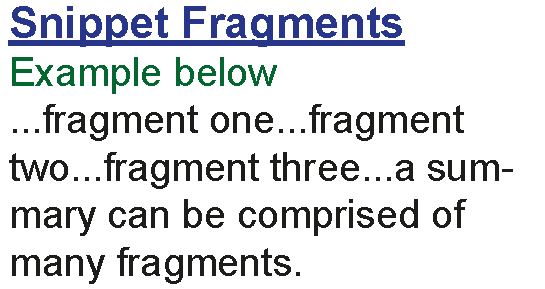
\includegraphics[width=1\textwidth]{figures/ch7-fragments.pdf}
    \end{center}
    \vspace*{-4mm}
    \label{fig:fragments}
\end{wrapfigure}

To decide the length and informativeness of the result summaries, we performed a preliminary analysis to determine the average length (in words) and informativeness (as calculated by the~\glsfirst{glos:kl}~\citep{kullback1951information} \todo{distance} to measure \emph{information gain}, or \emph{relative entropy}) of result summaries with the title, and a varying number of \emph{snippet fragments}\footnote{Figure~\ref{fig:serp_example} on page~\pageref{fig:serp_example} illustrates snippet fragments in the wider context of a~\gls{acr:serp}.} (from $0$ to $10$). The closer the entropy value is towards zero, the more information that is gained. Figure~\ref{fig:ig_plots} plots the number of words, the information gain, and the information gain attained per word.\footnote{These values were obtained by submitting over $300$ queries from a previous user study, conducted by~\cite{azzopardi2013query_cost}. These were conducted on similar topics, the same retrieval system and corpus used as the those used for this study.} It is clear from the plots shown in Figure~\ref{fig:ig_plots} that a higher level of information gain was present in longer snippets. However, as the length increased with each snippet fragment added, the informativeness per word also decreased. Consequently, we selected the four different interface conditions in the region where informativeness has the highest change, i.e. from zero to four. The conditions selected for this study were therefore:

\begin{figure}[t!]
    \centering
    \resizebox{1\hsize}{!}{
    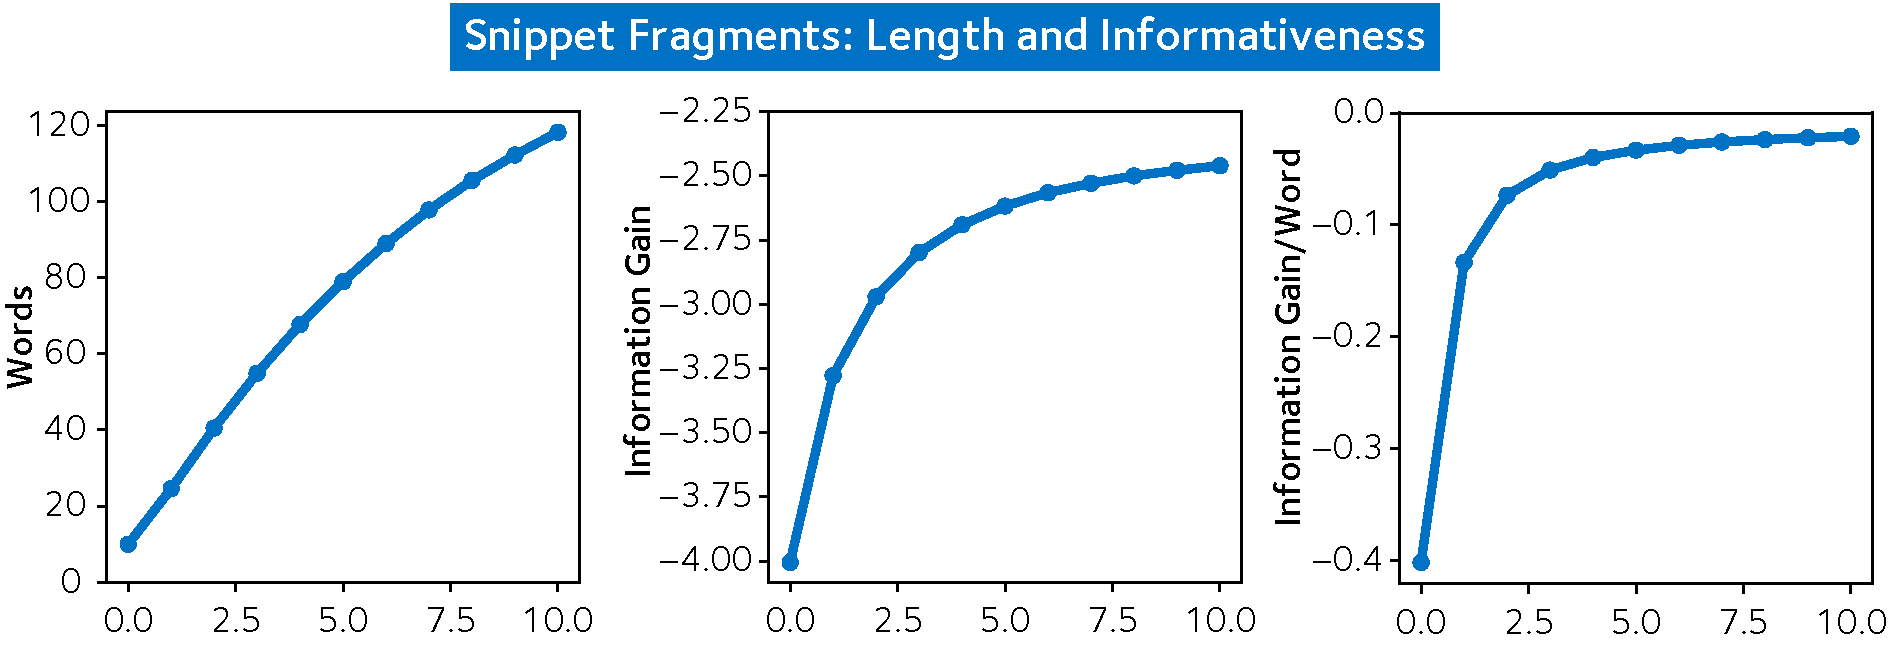
\includegraphics{figures/ch7-ig_plots.pdf}}
    \caption[Information gain plots]{Plots showing the length (in words), informativeness (in information gain, or \emph{IG}), and the information gain \emph{(IG)} per word for the title, plus 0 to 10 snippet fragments. The closer the value is to zero, the more information that is gained.}
    \label{fig:ig_plots}
\end{figure}

\begin{itemize}
    \item{\blueboxbold{T0}, where only the title for each result summary were presented;}
    \item{\blueboxbold{T1}, where for each result summary, a title and one query-biased snippet fragment were presented;}
    \item{\blueboxbold{T2}, where a title and two query-biased snippet fragments were presented; and}
    \item{\blueboxbold{T4}, where a title and four query-biased snippet fragments were presented.}
\end{itemize}

For these interfaces, our independent variable was snippet informativeness, controlled by the length of the result summary snippets. Figure~\ref{fig:interface_snippets} provides a complete, rendered example of the different result summaries in each condition, using the same document.

\begin{figure}[t!]
    \centering
    \resizebox{1\hsize}{!}{
    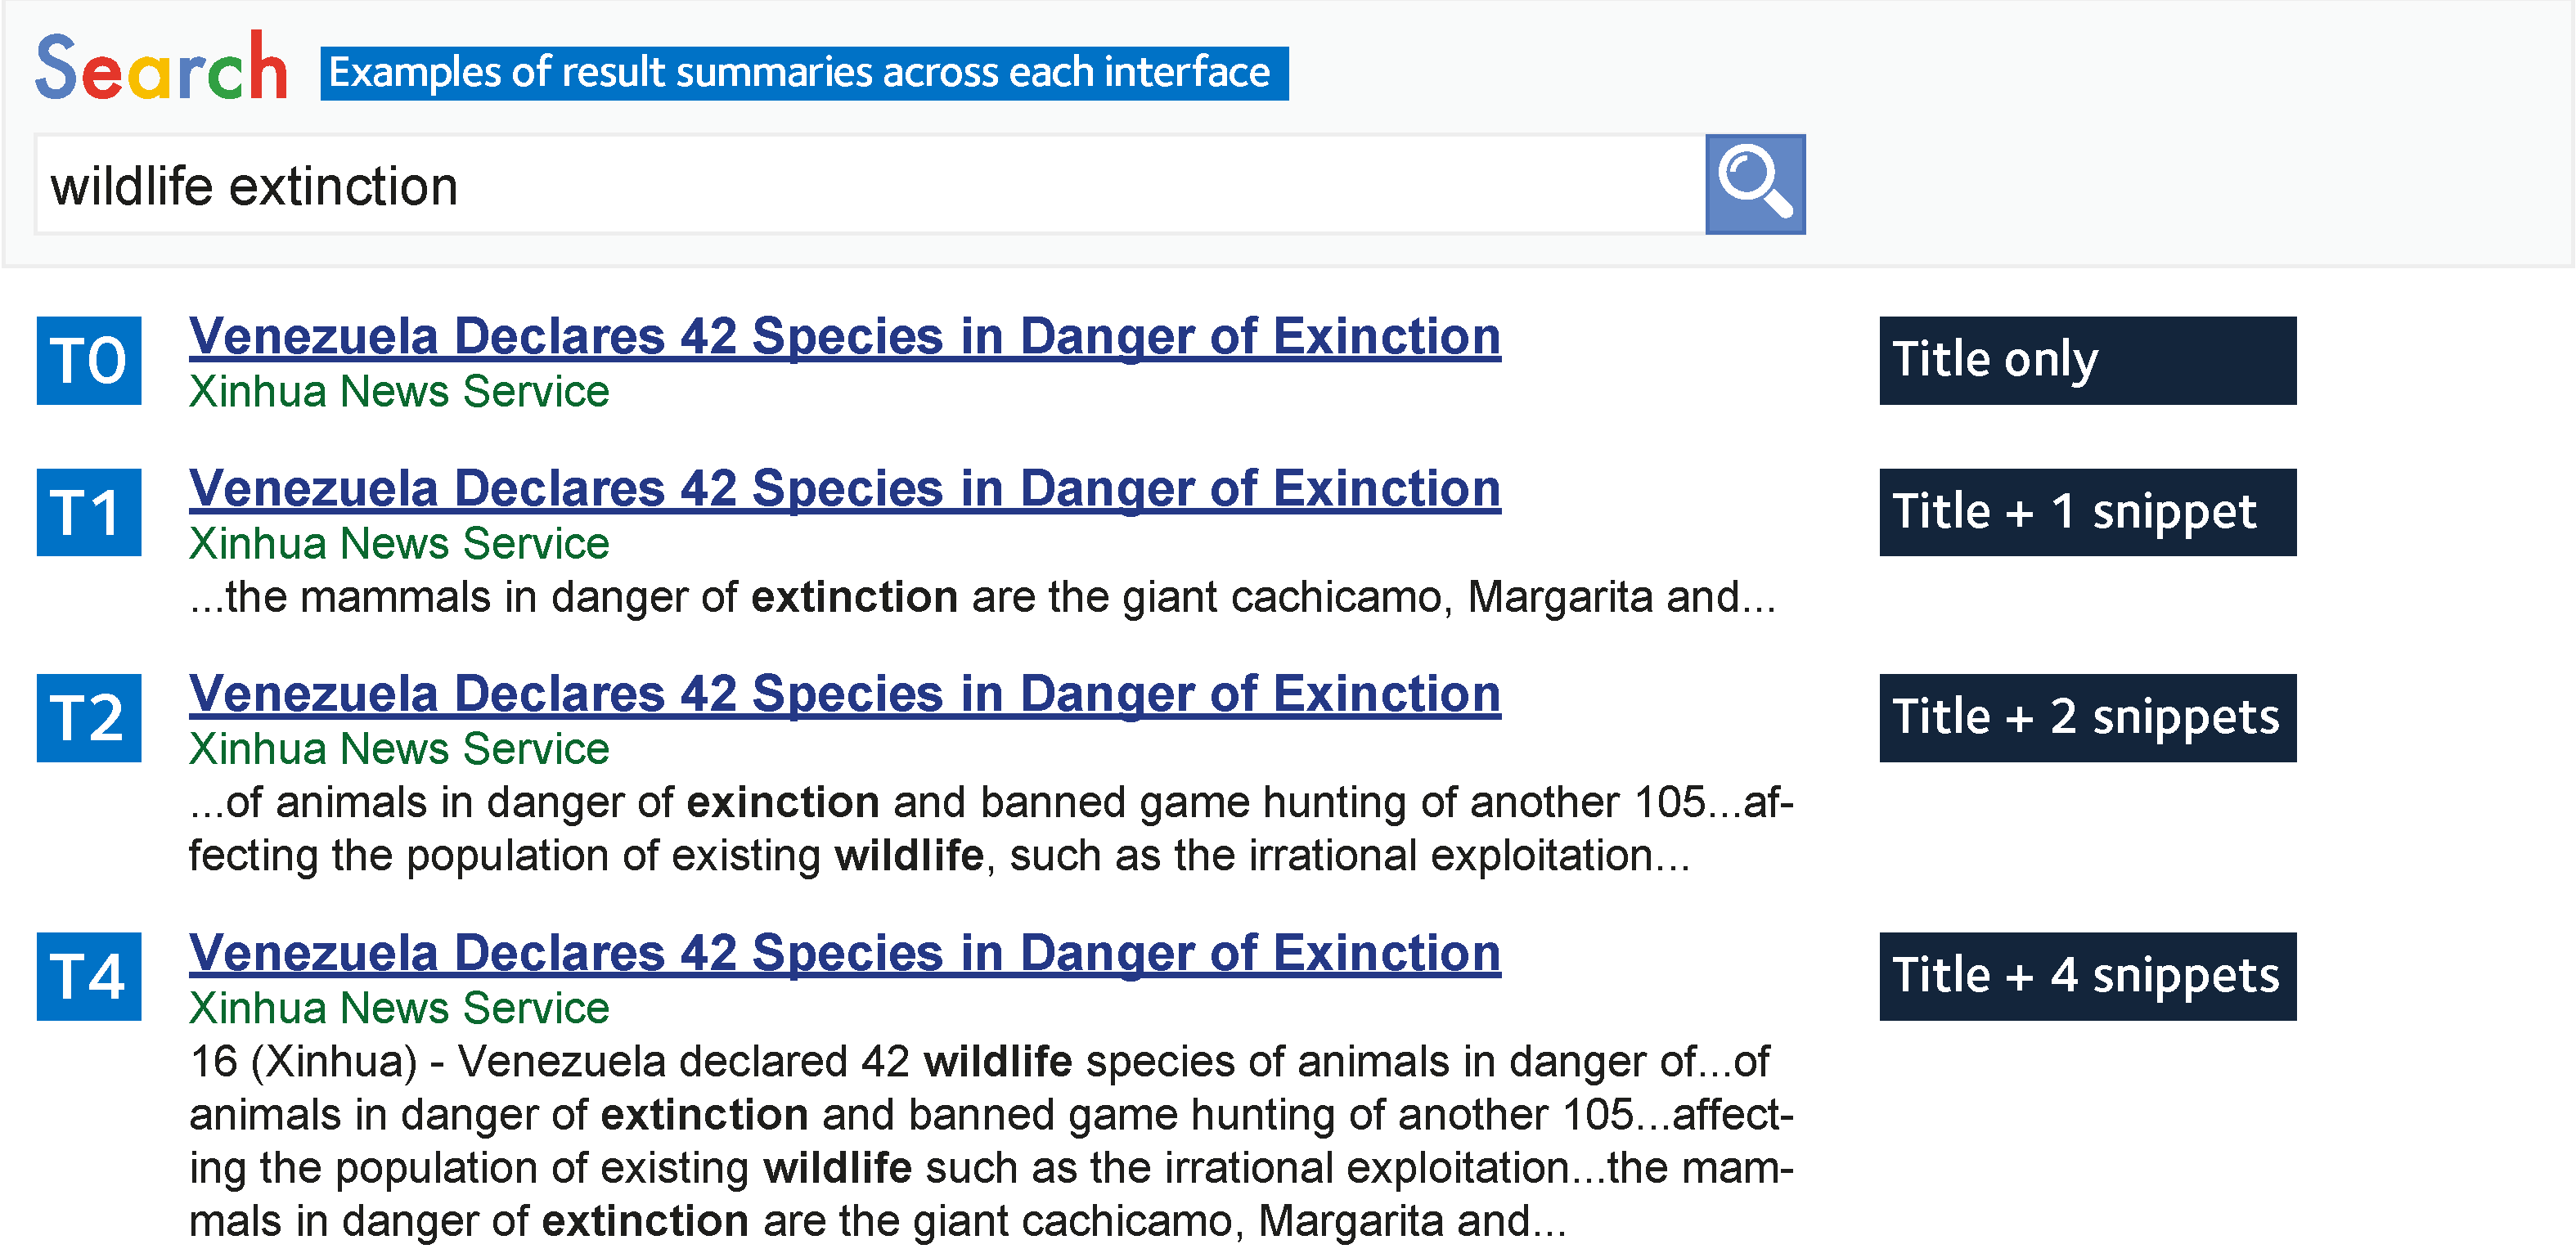
\includegraphics{figures/ch7-interface_snippets.pdf}}
    \caption[Examples of result summaries from the four interfaces]{Examples of the result summaries generated by each of the four interfaces, \blueboxbold{T0}, \blueboxbold{T1}, \blueboxbold{T2} and \blueboxbold{T4} used in this study. The same document is used. Demonstrated by \searchlogo, each of the result summaries consists of: a title (in blue, underlined); none, one, or more snippet fragments (in black, with fragments separated by ellipses); and a newswire source (in green).}
    \label{fig:interface_snippets}
\end{figure}

From here, we carefully selected the order in which subjects were presented with each interface. For each of the four main topics discussed in Section~\ref{sec:methodology:collection:topics}, one of the four interfaces from \blueboxbold{T0}, \blueboxbold{T1}, \blueboxbold{T2} and \blueboxbold{T4} were assigned to a topic using a Latin-square rotation. For the practice topic, we used \blueboxbold{T2} -- a title and two snippet fragments -- the interface that represented the \emph{de facto} standard for presenting result summaries~\citep{hearst2009_search}.

\subsubsection{Snippet Generation}\label{sec:snippets:method:snippets}
For interfaces \blueboxbold{T2} to \blueboxbold{T4}, each result summary presented to the subjects required one or more snippet fragments from the corresponding document. As illustrated in the complete, rendered example in Figure~\ref{fig:interface_snippets}, each of the fragments generated were query-biased~\citep{tombros1998query_biased} in nature. Fragments were generated by splitting a given document into sentences (delimited by a full stop), and scoring each of the sentences according to BM25 (where $\beta=0.75$). Fragments were then extracted from the ordered series of sentences by identifying query terms within those sentences, with a window of $40$ characters from either side of the query term.

\begin{figure}[h]
    \centering
    \vspace{4mm}
    \resizebox{1\hsize}{!}{
    
\includegraphics{figures/ch7-fragment_example.pdf}}
    \label{fig:fragment_example}
    \vspace{-5mm}
\end{figure}

The ordered set of fragments were then joined together (one only for \blueboxbold{T1}, two for \blueboxbold{T2}, and four for \blueboxbold{T4}), separated by ellipses. These were combined together with the document's title and source newswire to form the complete result summary.

\subsubsection{Search Task}
As discussed previously in Section~\ref{sec:methodology:user:flow}, subjects were grounded by instructing them to imagine that they were newspaper reporters. As such, they were required to gather documents to write stories about each of the four topics they searched for. For this study, subjects were assigned ten minutes to each of the four search tasks, and were specifically instructed to find as many relevant documents as they could during this allotted time. As shown in Section~\ref{sec:methodology:user:interface}, subjects interacted with the standard search interface. Documents were \emph{saved} by subjects when they were considered to be relevant to the given~\gls{acr:trec} topic.

\subsubsection{Crowdsourced Subjects}\label{sec:snippets:method:subjects}
A total of $60$ subjects took part on the~\gls{acr:mturk} platform between July and August, 2016. However, seven subjects were omitted due to quality control constraints imposed on the study -- refer to Section~\ref{sec:methodology:user:crowdsourcing} for more information on the constrains imposed. This left $53$ subjects who satisfied the conditions of the experiment. In all, of the $53$ subjects who satisfied the criteria, $28$ were male, with the remaining $25$ female. The average age of the subjects was $33.8$ years ($min=22$; $max=48$; $stdev=7.0$). A total of $19$ subjects reported possessing a bachelor's degree or higher, and all expressing a high degree of search literacy, and conducted at least five searches for information online per week.

With a total of $53$ subjects considered in the results of this study, each searching over four topics, this meant a total of $212$ search sessions being logged and available for analysis. Finally, we report results over a reduced time period of six minutes ($360$ seconds). This decision was taken as not all of the $53$ subjects spent the full ten minutes searching, with these subjects skewing results. By reducing the time period that we considered, we ensured that we could extract meaningful data from the interaction logs, where all subjects were interacting with the experimental system.

\subsubsection{Post-Task Surveys}\label{sec:snippets:method:posttask}
With the pre-task survey the same as that outlined in the general methodology (refer to Section~\ref{sec:methodology:extracting}), surveys for this study differed post-task and post-experiment. Here, we discuss the questions posed in each of the four post-task surveys.

A seven-point Likert scale was used for post-task surveys, similar to the pre-task surveys. Upon completion of each search task, the following statements were completed by each subject, selecting from \emph{strongly disagree} to \emph{strongly agree.}

\begin{itemize}
    \item{\blueboxbold{Clarity} The result summaries presented were clear and concise.}
    \item{\blueboxbold{Confidence} The result summaries presented increased my confidence in my decisions.}
    \item{\blueboxbold{Informativeness} The result summaries presented were informative to me.}
    \item{\blueboxbold{Relevance} The result summaries presented allowed me to judge the relevance of the associated document.}
    \item{\blueboxbold{Readability} The result summaries presented were readable.}
    \item{\blueboxbold{Size} The result summaries presented were of an appropriate size and length.}
\end{itemize}

These questions allowed us to obtain quantitative data alluding to how each subject perceived the search interface that they interacted with, and ascertain what they thought of the different result summary lengths.

\subsubsection{Post-Experiment Survey}\label{sec:snippets:method:postexperiment}
At the end of the experiment, subjects also completed a post-experiment survey. Five questions were posed, this time asking subjects to select which one of the four different interfaces best matched up with their opinion of the question asked.

\begin{itemize}
    \item{\blueboxbold{Most Informative?} Of the four interfaces, what one yielded the most informative result summaries?}
    \item{\blueboxbold{Least Helpful?} Of the four interfaces, which one provided the most unhelpful result summaries?}
    \item{\blueboxbold{Easiest?} Which of the four interfaces provided result summaries that were easiest to understand?}
    \item{\blueboxbold{Least Useful?} Of the four interfaces, which one provided the least useful result summaries?}
    \item{\blueboxbold{Most Preferred?} Of the four interfaces, what interface did you prefer using the most?}
\end{itemize}

These questions allowed us to determine which interface delivered the best impression overall across the five different questions asked.

\subsection{Results and Analysis}\label{chap:snippets:user:results}
From the four aspects we highlighted in Section~\ref{sec:methodology:extracting}, we report results from the study across four main sections, including analysis of: \emph{(i)} behavioural measures (interactions); \emph{(ii)} time-based measures; \emph{(iii)} performance measures; and finally \emph{(iv)} user experience (surveys). Each measure was analysed over the four different search interfaces. To perform our analysis, \emph{Analysis of Variance (ANOVA) tests} were used using the interfaces as factors; main effects were examined with $\alpha = 0.05$. Bonferroni tests were used for post-hoc analysis.

\begin{table}[t!]
    \caption[Information gain across interfaces]{Characters, words and \emph{Information Gain (IG)} across each of the four interfaces trialled. An ANOVA test revealed significant differences, with follow-up tests showing that each interface is significantly different to others. An IG value closer to zero denotes a higher level of IG. In the table below, \emph{IG/W.} denotes \emph{IG per word}.\vspace{-3mm}}
    \label{tbl:snippets_info_gain}
    \renewcommand{\arraystretch}{1.8}
    \begin{center}
    \begin{tabulary}{\textwidth}{L{3.75cm}@{\CS}D{2.6cm}@{\CS}D{2.6cm}@{\CS}D{2.6cm}@{\CS}D{2.6cm}}
    
    \RS & \lbluecell\textbf{\emph{T0}} & \lbluecell\textbf{\emph{T1}} & \lbluecell\textbf{\emph{T2}} & \lbluecell\textbf{\emph{T4}}\\
    % OUTPUT FROM script
    
    \RS\lbluecell\textbf{Words} & \cell6.58$\pm$0.01* & \cell25.21$\pm$0.06* & \cell44.29$\pm$0.10* & \cell77.06$\pm$0.13* \\
    \RS\lbluecell\textbf{Characters} & \cell37.37$\pm$0.05* & \cell103.29$\pm$0.17* & \cell168.36$\pm$0.23* & \cell284.78$\pm$0.31* \\
    \RS\lbluecell\textbf{IG} & \cell-6.35$\pm$0.01* & \cell-3.59$\pm$0.00* & \cell-3.00$\pm$0.00* & \cell-2.67$\pm$0.00* \\
    \RS\lbluecell\textbf{IG/Word} & \cell-1.17$\pm$0.00* & \cell-0.18$\pm$0.00* & \cell-0.08$\pm$0.00* & \cell-0.04$\pm$0.00* \\
    
\end{tabulary}
\end{center}
\end{table}

To check whether the interfaces were sufficiently different with respect to snippet length and information gain, we performed an analysis of the result summaries that were presented to the subjects. Table~\ref{tbl:snippets_info_gain} summarises, over each interface, the number of words and characters that result summaries contained on average. As expected, the table shows an increasing trend of words and characters as the number of snippet fragments were increased. Information gain (or relative entropy), as previously discussed, was calculated using~\gls{glos:kl}~\citep{kullback1951information}. Statistical testing showed that the differences between snippet length ($F(3,208 = 1.2x10^5, p<0.001)$) and information gain ($F(3,208) = 2.6x10^5, p<0.001)$) were significant. Follow up tests revealed that this was the case over all four interfaces, indicating that our conditions were indeed different on these dimensions. These findings provide some justification for our choices of the number of snippet fragments used with each interface. A diminishing increase in information gain after four snippet fragments suggested that there would not have been much point generating result summaries that were any longer.

\begin{table}[t!]
    \caption[Behaviour and performance over experimental interfaces]{Various measures reported over each of the four experimental interfaces, \blueboxbold{T0}, \blueboxbold{T1}, \blueboxbold{T2} and \blueboxbold{T4}. Included are interaction and time-based measures (behavioural), as well as performance-based measures. No significant differences were observed, bar for the time per result summary. Refer to Section~\ref{chap:snippets:user:results:time} for details.}
    \label{tbl:snippets_intperftime}
    \renewcommand{\arraystretch}{1.8}
    \begin{center}
    \begin{tabulary}{\textwidth}{L{0.4cm}@{\CS}L{3.2cm}@{\CS}D{2.5cm}@{\CS}D{2.5cm}@{\CS}D{2.5cm}@{\CS}D{2.5cm}@{\CS}}

        \RS & & \lbluecell \textbf{T0} & \lbluecell \textbf{T1} & \lbluecell \textbf{T2} & \lbluecell \textbf{T4} \\

        \RS \multirow{4}{*}{\rotatebox{90}{\hspace*{-5mm}\textbf{Interactions}}} & \lbluecell\textbf{\#Queries} & \cell \small{3.72$\pm$0.34} & \cell \small{3.19$\pm$0.35} & \cell \small{3.30$\pm$0.35} & \cell \small{3.28$\pm$0.31}\\
        \RS & \lbluecell\textbf{\#\glsplural{acr:serp}/Query} & \cell \small{2.87$\pm$0.29} & \cell \small{2.69$\pm$0.23} & \cell \small{2.43$\pm$0.13} & \cell \small{2.40$\pm$0.20}\\
        \RS & \lbluecell\textbf{\#Docs./Query} & \cell \small{4.23$\pm$0.55} & \cell \small{4.83$\pm$0.54} & \cell \small{5.14$\pm$0.66} & \cell \small{4.76$\pm$0.62}\\
        \RS & \lbluecell\textbf{Depth/Query} & \cell \small{24.47$\pm$2.96} & \cell \small{22.87$\pm$2.47} & \cell \small{20.02$\pm$1.46} & \cell \small{19.40$\pm$2.04}\\
        
        \RS\RS\RS \multirow{4}{*}{\rotatebox{90}{\hspace*{-5mm}\textbf{Performance}}} & \lbluecell\textbf{P@10} & \cell \small{0.25$\pm$0.02} & \cell \small{0.23$\pm$0.02} & \cell \small{0.27$\pm$0.02} & \cell \small{0.25$\pm$0.03}\\
        \RS & \lbluecell\textbf{\#Saved} & \cell \small{6.68$\pm$0.66} & \cell \small{7.00$\pm$0.63} & \cell \small{6.49$\pm$0.58} & \cell \small{7.60$\pm$0.79}\\
        \RS & \lbluecell\textbf{\#\gls{acr:trec} Saved} & \cell \small{2.58$\pm$0.34} & \cell \small{2.28$\pm$0.25} & \cell \small{2.47$\pm$0.28} & \cell \small{2.66$\pm$0.32}\\
        \RS & \lbluecell\textbf{\#\gls{acr:trec} Non.} & \cell \small{1.85$\pm$0.32} & \cell \small{2.08$\pm$0.29} & \cell \small{1.98$\pm$0.24} & \cell \small{1.68$\pm$0.32}\\
        
        \RS\RS\RS \multirow{3}{*}{\rotatebox{90}{\hspace*{-5mm}\textbf{Times}}} & \lbluecell\textbf{Per Query} & \cell \small{8.29$\pm$0.57} & \cell \small{7.99$\pm$0.57} & \cell \small{9.42$\pm$0.79} & \cell \small{8.12$\pm$0.48}\\
        \RS & \lbluecell\textbf{Per Document} & \cell \small{17.32$\pm$2.12} & \cell \small{22.82$\pm$6.03} & \cell \small{17.19$\pm$1.86} & \cell \small{18.99$\pm$2.13}\\
        \RS & \lbluecell\textbf{Per Summary} & \cell \small{1.63$\pm$0.13*} & \cell \small{2.21$\pm$0.21} & \cell \small{2.35$\pm$0.23} & \cell \small{2.60$\pm$0.27*}\\
        
    \end{tabulary}
    \end{center}
\end{table}

\subsubsection{Interaction Measures}
Across the four experimental interfaces trialled, Table~\ref{tbl:snippets_intperftime} presents the mean (and standard deviations) of:

\begin{itemize}
    \item{the number of queries issued \emph{(\#Queries);}}
    \item{the number of~\gls{acr:serp} viewed per query \emph{(\#\glsplural{acr:serp}/Query);}}
    \item{the number of documents viewed per query \emph{(\#Docs./Query);} and}
    \item{the mean click depth -- or stopping depth \emph{(Depth/Query).}}
\end{itemize}

These are all presented within the \genericblack{Interactions}~grouping. Across the four experimental interfaces of \blueboxbold{T0}, \blueboxbold{T1}, \blueboxbold{T2} and \blueboxbold{T4}, there were no significant differences reported between any of these measures. The number of queries issued follows a slight downward trend as the length of the result summaries (dictated by the interface conditions) increased ($3.72 \pm 0.34$ for \blueboxbold{T0}, to $3.28\pm0.31$ for \blueboxbold{T4}). This was also true for the number of~\glsplural{acr:serp} examined, and the number of documents examined per query. The depth to which subjects went to per query however follows a downward trend. As the length of each result summary increased, subjects were likely to go to shallower depths per query when examining result summaries ($24.47\pm2.96$ for \blueboxbold{T0}, to $19.4\pm20.04$ for \blueboxbold{T4}).

\begin{table}[t!]
    \caption[Interaction probabilities]{A summary of the various interaction probabilities over each of the four experimental interfaces examined. Note the increasing trends for each probability from \blueboxbold{T0} $\rightarrow$ \blueboxbold{T4}. Section~\ref{sec:method:simulation:grounding:judgements} on page~\pageref{sec:method:simulation:grounding:judgements} provides an explanation of the various probabilities listed here.}
    \label{tbl:snippets_probabilities}
    \renewcommand{\arraystretch}{1.8}
    \begin{center}
    \begin{tabulary}{\textwidth}{L{0.4cm}@{\CS}L{3.2cm}@{\CS}D{2.5cm}@{\CS}D{2.5cm}@{\CS}D{2.5cm}@{\CS}D{2.5cm}@{\CS}}

        \RS & & \lbluecell \textbf{T0} & \lbluecell \textbf{T1} & \lbluecell \textbf{T2} & \lbluecell \textbf{T4} \\

        \RS \multirow{3}{*}{\rotatebox{90}{\hspace*{-5mm}\textbf{Click}}} & \lbluecell\textbf{P(C)} & \cell \small{0.20$\pm$0.02} & \cell \small{0.25$\pm$0.02} & \cell \small{0.26$\pm$0.03} & \cell \small{0.28$\pm$0.03}\\
        \RS & \lbluecell\textbf{P(C|R)} & \cell \small{0.28$\pm$0.03} & \cell \small{0.34$\pm$0.03} & \cell \small{0.35$\pm$0.03} & \cell \small{0.40$\pm$0.04}\\
        \RS & \lbluecell\textbf{P(C|N)} & \cell \small{0.18$\pm$0.02} & \cell \small{0.23$\pm$0.02} & \cell \small{0.25$\pm$0.03} & \cell \small{0.24$\pm$0.03}\\
        
        \RS\RS\RS \multirow{3}{*}{\rotatebox{90}{\hspace*{-5mm}\textbf{Save}}} & \lbluecell\textbf{P(S)} & \cell \small{0.61$\pm$0.04} & \cell \small{0.68$\pm$0.04} & \cell \small{0.65$\pm$0.03} & \cell \small{0.71$\pm$0.03}\\
        \RS & \lbluecell\textbf{P(S|R)} & \cell \small{0.66$\pm$0.06} & \cell \small{0.69$\pm$0.05} & \cell \small{0.67$\pm$0.05} & \cell \small{0.66$\pm$0.05}\\
        \RS & \lbluecell\textbf{P(S|N)} & \cell \small{0.55$\pm$0.04} & \cell \small{0.65$\pm$0.04} & \cell \small{0.58$\pm$0.04} & \cell \small{0.67$\pm$0.04}\\
        
    \end{tabulary}
    \end{center}
\end{table}

Interaction probabilities all showed an increasing trend as result summary length increased over the four experimental interfaces, as shown in Table~\ref{tbl:snippets_probabilities}. Explanations for what each of the different probabilities represent can be found in Section~\ref{sec:method:simulation:grounding:judgements} on page~\pageref{sec:method:simulation:grounding:judgements}. Although no significant differences were observed over the four interfaces and the different probabilities examined, trends across all probabilities show an increase as result summary length increased. An increase of both the probability of clicking result summaries on the~\gls{acr:serp} ($P(C)$) and saving the associated documents ($P(S)$) as relevant were observed. When these probabilities are examined in more detail by separating the result summaries clicked and documents saved by their~\gls{acr:trec} relevancy, we see increasing trends for clicking and saving -- both for~\gls{acr:trec} relevant ($P(C|R)$ and $P(S|R)$ for clicking and saving, respectively), and~\gls{acr:trec} non-relevant documents ($P(C|N)$ and $P(M|N)$). This interesting finding shows that an increase in result summary length does not necessarily improve a subject's accuracy, but simply the likelihood that they will consider documents to be relevant.


\subsubsection{Time-Based Measures}\label{chap:snippets:user:results:time}
Table~\ref{tbl:snippets_intperftime} also presents three time-based measures (within the \genericblack{Times}~grouping) that were observed across the four experimental interfaces. We show:

\begin{itemize}
    \item{the mean time spent by subjects issuing queries \emph{(Per Query);}}
    \item{the mean time spent by subjects examining individual documents \emph{(Per Document);} and}
    \item{the mean time spent by subjects examining individual result summaries \emph{(Per Summary).}}
\end{itemize}

\begin{figure}[t!]
    \centering
    \resizebox{1\hsize}{!}{
    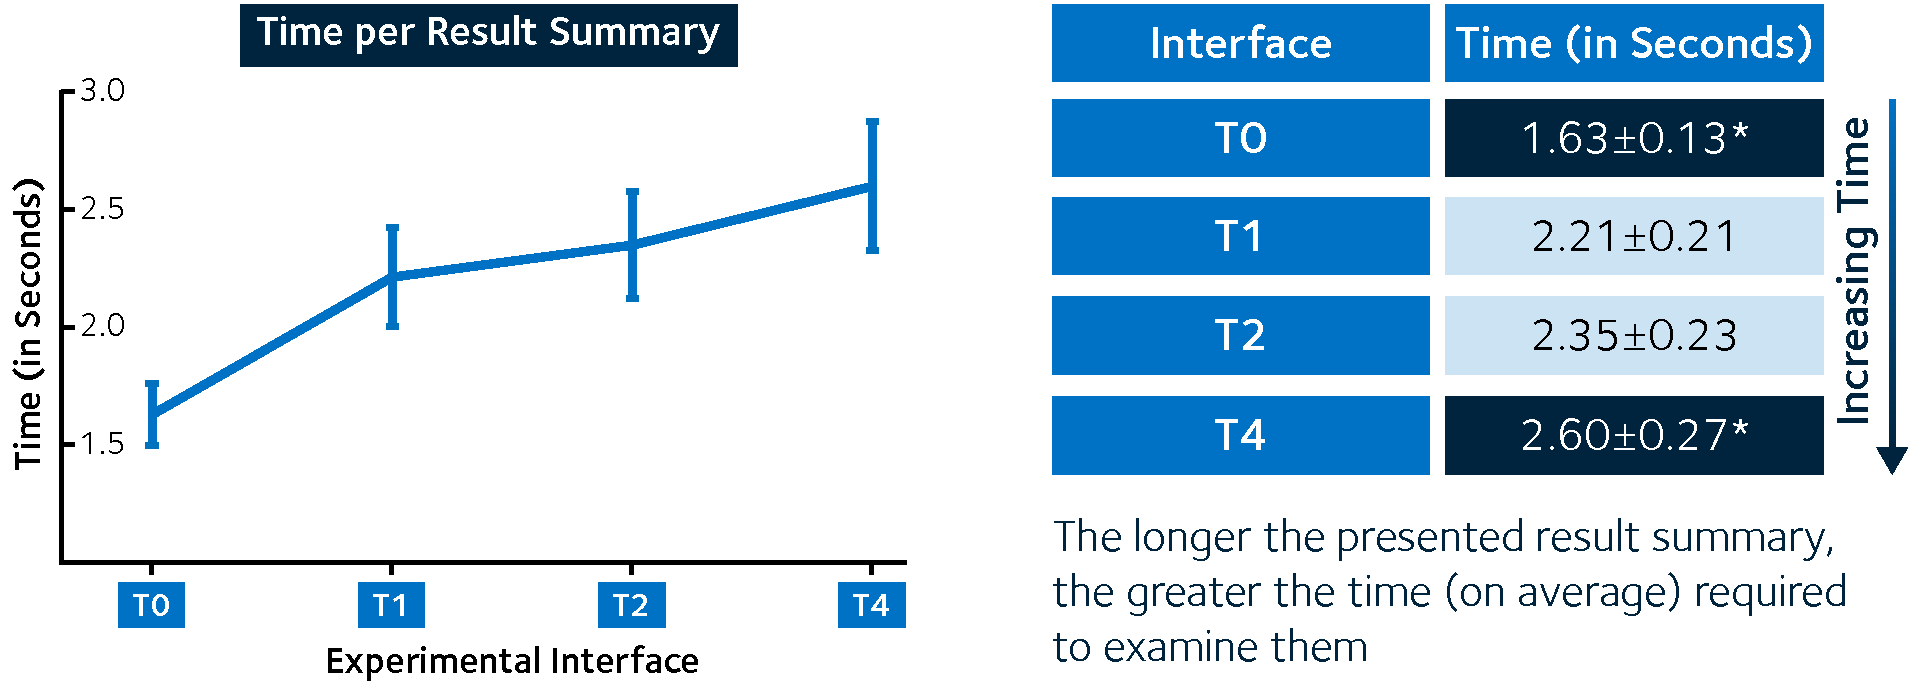
\includegraphics{figures/ch7-time_snippet.pdf}}
    \caption[Time per result summary]{Plot and table illustrating the mean time spent examining result summaries across each of the four experimental interfaces trialled. Note the increasing mean examination time as the result summary length increases, from \blueboxbold{T0} $\rightarrow$ \blueboxbold{T4}. Error bars denote the standard deviation.}
    \label{fig:time_snippet}
\end{figure}

No significant differences were found between the time spent per query, and the time spent examining individual documents. However, a significant difference did exist for the time spent per result summary, as can be seen from the table. A clear upward trend in the time spent examining result summaries can be seen in Figure~\ref{fig:time_snippet} as result summaries progressively got longer, from $1.63\pm0.13$ for \blueboxbold{T0} to $2.6\pm0.27$ for \blueboxbold{T4}, which was significantly different ($F(3,208) = 3.6, p=0.014$). The follow-up Bonferroni test showed that the significant difference did exist between interfaces \blueboxbold{T0} and \blueboxbold{T4}. This finding suggests that as result summary length increases, the amount of time spent examining individual result summaries also increases, presenting us with an intuitive result. This also complies with trends observed regarding examination depths. When the length of result summaries increased, subjects were likely to examine result summaries to shallower depths.

\subsubsection{Performance}
Also included within Table~\ref{tbl:snippets_intperftime} are our reported performance measures, this time shown under the \genericblack{Performance}~grouping. Again, these are reported over each of the four experimental interfaces trialled. We report the mean performance of:

\begin{itemize}
    \item{the issued queries, with the $P@10$ score;}
    \item{the number of documents that were saved by subjects \emph{(\#Saved);}}
    \item{the interactive precision, or the number of saved documents that were~\gls{acr:trec} relevant \emph{(\#\gls{acr:trec} Saved);} and also}
    \item{the number of saved documents that were not~\gls{acr:trec} relevant \emph{(\#\gls{acr:trec} Non.).}}
\end{itemize}

Like the interaction measures examined previously, no significant differences were observed over the four experimental interfaces examined. The performance of queries issued by subjects was very similar across all interfaces ($P@10 \approx 0.25$), along with the number of documents identified by subjects as relevant ($6.49\pm0.58$) for \blueboxbold{T2} to $7.6\pm0.79$ for \blueboxbold{T4}, and the interactive precision ($2.28\pm0.25$ for \blueboxbold{T1} to $2.66\pm0.32$ for \blueboxbold{T4}). Considering the number of saved,~\gls{acr:trec} non-relevant documents, where subjects on averaged saved two such documents. However, there again no significant differences between the four interfaces.

\subsubsection{User Experience}\label{chap:snippets:user:results:ux}
In this section, we analyse the results of the post-task and post-experiment surveys that subjects completed. Examining the results from these surveys allow us to capture the subject's perceived experiences of using the experimental system across all four interfaces trialled.

\begin{table}[t!]
    \caption[Post-task survey results]{Summary table of the recorded observations for the post-task surveys, indicating the preferences of subjects over the six criteria and four experimental interfaces. Across all criteria, \blueboxbold{T0} was significantly different from the other three interfaces (denoted by *). Using the seven-point Likert scale, results are shown from 1 (strongly disagree) to 7 (strongly agree).}
    \label{tbl:snippets_posttask}
    \renewcommand{\arraystretch}{1.8}
    \begin{center}
    \begin{tabulary}{\textwidth}{L{4.15cm}@{\CS}D{2.5cm}@{\CS}D{2.5cm}@{\CS}D{2.5cm}@{\CS}D{2.5cm}@{\CS}}

        \RS & \lbluecell \textbf{T0} & \lbluecell \textbf{T1} & \lbluecell \textbf{T2} & \lbluecell \textbf{T4} \\

        \RS \lbluecell\textbf{Clarity} & \cell \small{4.16$\pm$0.27*} & \cell \small{5.00$\pm$0.21} & \cell \small{5.06$\pm$0.24} & \cell \small{5.40$\pm$0.20}\\
        \RS \lbluecell\textbf{Confidence} & \cell \small{3.71$\pm$0.26*} & \cell \small{4.66$\pm$0.26} & \cell \small{4.75$\pm$0.24} & \cell \small{5.06$\pm$0.25}\\
        \RS \lbluecell\textbf{Informativeness} & \cell \small{4.20$\pm$0.30*} & \cell \small{5.38$\pm$0.24} & \cell \small{5.27$\pm$0.24} & \cell \small{5.62$\pm$0.20}\\
        \RS \lbluecell\textbf{Relevance} & \cell \small{3.84$\pm$0.28*} & \cell \small{4.89$\pm$0.25} & \cell \small{5.08$\pm$0.24} & \cell \small{5.36$\pm$0.20}\\
        \RS \lbluecell\textbf{Readability} & \cell \small{5.18$\pm$0.31*} & \cell \small{6.32$\pm$0.17} & \cell \small{6.46$\pm$0.14} & \cell \small{6.36$\pm$0.14}\\
        \RS \lbluecell\textbf{Size} & \cell \small{4.00$\pm$0.31*} & \cell \small{4.94$\pm$0.25} & \cell \small{5.21$\pm$0.22} & \cell \small{5.36$\pm$0.19}\\
        
    \end{tabulary}
    \end{center}
\end{table}

\blueboxheader{Post-Task Surveys}
Table~\ref{tbl:snippets_posttask} presents the mean set of results (and their standard deviations) from subjects across the four interfaces trialled. As previously discussed, these questions were answered upon the completion of each search task. The survey questions are detailed in Section~\ref{sec:snippets:method:posttask}. Using a seven-point Likert scale for their responses (with $1$ denoting a strong disagreement, and $7$ denoting a strong agreement), significant differences were found in all question responses, as shown below.

\begin{itemize}
    \item{\blueboxbold{Clarity} $F(3,208)=5.22, p=0.001$}
    \item{\blueboxbold{Confidence} $F(3,208)=5.2, p=0.001$}
    \item{\blueboxbold{Informativeness} $F(3,208)=5.22, p=0.001$}
    \item{\blueboxbold{Relevance} $F(3,208)=6.44, p<0.001$}
    \item{\blueboxbold{Readability} $F(3,208)=9.25, p<0.001$}
    \item{\blueboxbold{Size} $F(3,208)=7.28, p<0.001$}
\end{itemize}

Follow-up Bonferroni tests however shows that the significant difference existed only between \blueboxbold{T0} and the remaining three interfaces, \blueboxbold{T1}, \blueboxbold{T2} and \blueboxbold{T4}. A series of discernible trends can be observed throughout the responses, with subjects regarding longer result summaries as more concise, and a possessing a higher degree of clarity ($4.16\pm0.27$ for \blueboxbold{T0} to $5.4\pm0.2$ for \blueboxbold{T4}). This perceived clarity also made subjects feel more confidence that the longer result summaries helped them make better decisions as to whether they were relevant to the given topic. Interaction results presented above however differ from this (as shown in Table~\ref{tbl:snippets_probabilities}), where the overall probability of saving documents increased, regardless of the document/topic relevancy judgement. Other notable trends observed from the results included an increase in how informative subjects perceived results to be -- again, with longer result summaries proving to be more informative. Subjects also reported a general increase in satisfaction of the length of the presented result summaries. However, as mentioned, no significant difference existed between the three interfaces in which snippets were generated as part of the result summaries (i.e. \blueboxbold{T1}, \blueboxbold{T2} and \blueboxbold{T4}).

\blueboxheader{Post-Experiment Survey}
As detailed previously in Section~\ref{sec:snippets:method:postexperiment}, subjects completed a post-experiment exit survey. Responses from the subjects are presented in Table~\ref{tbl:snippets_postexp}. From the results, subjects found result summaries of longer lengths (i.e. those generated by interfaces \blueboxbold{T2} and \blueboxbold{T4}) to be the most informative, and those generated by \blueboxbold{T0} -- without any snippet(s) -- to be the least helpful and useful. The longer result summaries were also consistently favoured by subjects who preferred them over the result summaries generated by interfaces \blueboxbold{T0} and \blueboxbold{T1}. Subjects also found the result summaries of longer length easier to use to satisfy the given information need.

From the results, it is therefore clear that a majority of subjects preferred longer result summaries to be presented on~\glsplural{acr:serp}, generated by interfaces \blueboxbold{T2} and \blueboxbold{T4}.

\begin{table}[t!]
    \caption[Post-experiment survey results]{Raw results presenting responses from the post-experiment exit survey completed by each subject. More information on the survey can be found in SectionSection~\ref{sec:snippets:method:postexperiment}, with results discussed in Section~\ref{chap:snippets:user:results:ux}.}
    \label{tbl:snippets_postexp}
    \renewcommand{\arraystretch}{1.8}
    \begin{center}
    \begin{tabulary}{\textwidth}{L{4.15cm}@{\CS}D{2.5cm}@{\CS}D{2.5cm}@{\CS}D{2.5cm}@{\CS}D{2.5cm}@{\CS}}

        \RS & \lbluecell \textbf{T0} & \lbluecell \textbf{T1} & \lbluecell \textbf{T2} & \lbluecell \textbf{T4} \\

        \RS \lbluecell\textbf{Most Informative} & \cell \small{1} & \cell \small{4} & \cell \small{\textbf{20}} & \cell \small{\textbf{29}}\\
        \RS \lbluecell\textbf{Least Helpful} & \cell \small{\textbf{46}} & \cell \small{5} & \cell \small{1} & \cell \small{2}\\
        \RS \lbluecell\textbf{Easiest} & \cell \small{4} & \cell \small{4} & \cell \small{\textbf{24}} & \cell \small{\textbf{22}}\\
        \RS \lbluecell\textbf{Least Useful} & \cell \small{\textbf{49}} & \cell \small{4} & \cell \small{0} & \cell \small{1}\\
        \RS \lbluecell\textbf{Most Preferred} & \cell \small{3} & \cell \small{5} & \cell \small{\textbf{20}} & \cell \small{\textbf{26}}\\
        
    \end{tabulary}
    \end{center}
\end{table}

\subsection{Discussion and User Study Conclusions}
This user study investigated the influence of result summary length on search behaviour and performance. Using Kullback-Leibler distance~\citep{kullback1951information} as a measure of information gain, we examined result summaries of different lengths, selected a series of result summary lengths (comprised of snippet fragments) where there was a significant difference in information gain between them, which yielded the configurations for our four experimental conditions, \blueboxbold{T0}, \blueboxbold{T1}, \blueboxbold{T2} and \blueboxbold{T4}. A crowdsourced, within-subjects user study was performed comprising of 53 subjects, each of whom undertook four search tasks, using each of the four experimental interfaces.

This work was focused around addressing the two key research questions, which explored \blueboxbold{RQ1} how the length of a result summary affected search behaviour and user experience; and \blueboxbold{RQ2} whether the length of result summaries affected the decision making ability and accuracy of the subjects. Addressing \blueboxbold{RQ1} first in terms of search behaviour, there was admittedly little difference -- but we did observe the following trends. As result summary length increased, subjects:

\begin{itemize}
    \item{issued fewer queries and examined fewer pages; \emph{but importantly}}
    \item{\emph{clicked more documents.}}
\end{itemize}

These findings demonstrate that subjects would spend more of their time assessing documents at higher ranks. Second, our results show that in terms of experience, subjects broadly preferred longer result summaries. The subjects felt that longer summaries were more clear, informative, readable -- and interestingly -- gave them more confidence in their relevance decisions.

With respect to \blueboxbold{RQ2}, we again observed little difference in subjects' decision making abilities and accuracy between the four experimental interfaces. While subjects perceived longer result summaries to help them infer relevance more accurately, our empirical evidence suggests otherwise. In fact, it would appear that longer result summaries were more attractive, increasing the information scent of the~\gls{acr:serp}. This may account for the increase in clicks on the early results, without the benefits, however: accuracy of our subjects did not improve with longer result summaries, nor did they find more relevant documents. Increased confidence in the result summaries (from interfaces \blueboxbold{T0} $\rightarrow$ \blueboxbold{T4}) may have led to a more relaxed approach at saving content as relevant -- as can be seen by increasing click and mark probabilities for both relevant and non-relevant content. It is also possible that the \emph{paradox of choice}~\citep{oulasvirta2009serp_size} could play a role in shaping a searcher's preferences. For example, in the interface with the longest result summaries, \blueboxbold{T4}, subjects viewed fewer results/choices than on other conditions. This may have contributed to their feelings of greater satisfaction and increased confidence in their decisions.

These novel findings provide new insights into how searchers interact with result summaries in terms of their experiences and search behaviours. Previous work had only focused upon task completion times and accuracy of the first result while not considering their experiences~\citep{cutrell2007eye_tracking, kaisser2008improving}. Our findings show that longer result summaries, while containing a greater amount of information content, are not necessarily better in terms of decision making -- although subjects perceived this to be the case. We also show a positive relationship between the length and informativeness of result summaries and their attractiveness (clickthrough rates). These results show that the experiences and perceptions of searchers -- and the actual performance of those searchers -- is different, and when designing interfaces, this needs to be taken into account.

Taking our findings from this user study, the next section discusses our simulation experiment, considering data from this user study as a means of grounding our simulations.

\section{Simulated Analysis}\label{sec:snippets:simulations}
We now move from the user study reported above to a simulated analysis, examining closely how stopping behaviour varies when searchers are subjected to result summaries of varying length. In particular, this section provides results and discussion of an extensive set of simulations, examining how the thirteen different snippet level stopping strategies (defined in Chapter~\ref{chap:strategies}):

\begin{itemize}
    \item{\blueboxbold{HL-RQ3a} perform; and}
    \item{\blueboxbold{HL-RQ3b} how closely they approximate actual searcher stopping behaviour.}
\end{itemize}

For both research questions, these are addressed under the context of what happens to performance and approximations when result summary lengths are varied. In the remainder of this section, we provide methodology details specific to this study (Section~\ref{sec:snippets:simulations:method}), before providing the results of the simulations (Section~\ref{sec:snippets:simulations:results}).

\subsection{Methodology}\label{sec:snippets:simulations:method}
This small methodology section outlines the details specific to this set of simulations. One can assume that any components not discussed here were instantiated as presented in the general simulation methodology, as discussed in Section~\ref{sec:method:simulation} on page~\pageref{sec:method:simulation}.

As we wish to examine how stopping behaviour varies when searchers are exposed to interfaces yielding result summaries of different lengths, we utilised all four of the experimental interfaces discussed previously in this simulation study. Below, we discuss the interfaces used (Section~\ref{sec:snippets:simulations:method:interfaces}), before outlining the interaction costs and probabilities extracted for each interface (Section~\ref{sec:method:simulation:grounding:costs}).

\subsubsection{Experimental System and Interfaces}\label{sec:snippets:simulations:method:interfaces}
The experimental system used for these simulations was largely the same as outlined in Section~\ref{sec:method:simulation} on page~\pageref{sec:method:simulation} -- save for the incorporation of the snippet generation components as outlined previously in Section~\ref{sec:snippets:method:snippets} within the \simiir~framework.

By incorporating this component, this allowed us to run simulations that presented to simulated searchers four different interfaces, namely \blueboxbold{T0}, \blueboxbold{T1}, \blueboxbold{T2}, and \blueboxbold{T4}. This allowed us to mirror as closely as possible -- given the experimental setup -- the interfaces that the real-world searchers were subjected to in the associated user study.

\subsubsection{Interaction Costs and Probabilities}\label{sec:snippets:simulations:method:costs}
We then took the interaction log data from the associated user study. For each of the four experimental interfaces trialled in the user study, we could then, following the methodology outlined in Sections~\ref{sec:method:simulation:grounding:judgements} and~\ref{sec:method:simulation:grounding:costs}, extract the different interaction probabilities and costs to ground our simulations.

The interaction probabilities and costs for each of the four interfaces are presented in Table~\ref{tbl:snippets_simulation_probcosts}. Included in the table under the \genericblack{P(C)} and \genericblack{P(S)} groupings are:

\begin{itemize}
    \item{the probabilities for clicking a result summary link, broken down over whether the associated document is~\gls{acr:trec} relevant ($P(C|R)$) or not ($P(C|N)$); and}
    \item{the probabilities for saving a document (denoting its relevance to the given~\gls{acr:trec} topic), again broken down over whether the document is~\gls{acr:trec} relevant ($P(S|R)$) or not ($P(S|N)$).}
\end{itemize}

Interaction costs denote the time required by simulated searchers to undertake different tasks. The interaction costs considered and listed in Table~\ref{tbl:snippets_simulation_probcosts} (under the \genericblack{Costs} grouping) include:

\begin{itemize}
    \item{the time taken to issue a query;}
    \item{the time taken to perform an initial examination of the~\gls{acr:serp};}
    \item{the time taken for a simulated searcher to examine an individual result summary;}
    \item{the time taken for a document examination; and}
    \item{the time required to save a document.}
\end{itemize}

Details for what constitutes each individual interaction cost can be found, as previously stated, in Section~\ref{sec:method:simulation:grounding:costs} on page~\pageref{sec:method:simulation:grounding:costs}. Note that the~\gls{acr:serp} examination cost is included even though the~\gls{acr:serp} stopping decision point is disabled in these simulations; this ensures that a cost is still paid, meaning that the interaction times stay realistic. Regarding total session time, simulated searchers were permitted a total of $360$ seconds to perform each search session -- the same session time used in the user study analysis, as discussed in Section~\ref{sec:snippets:method:subjects}.

\begin{table}[t!]
    \caption[Simulation interaction probabilities and costs]{Summary table of the different interaction costs (in seconds) and probabilities, with \emph{P(C)} denoting the probability of a click, and \emph{P(S)} denoting the probability of saving a document (considering it relevant). Refer to Sections~\ref{sec:method:simulation:grounding:costs} and~\ref{sec:method:simulation:grounding:judgements} respectively for further information on how the costs and probabilities were derived. All data in this table is attained from interaction data extracted from the user study reported in Section~\ref{chap:snippets:user}.}
    \label{tbl:snippets_simulation_probcosts}
    \renewcommand{\arraystretch}{1.8}
    \begin{center}
    \begin{tabulary}{\textwidth}{L{0.4cm}@{\CS}L{3.2cm}@{\CS}D{2.5cm}@{\CS}D{2.5cm}@{\CS}D{2.5cm}@{\CS}D{2.5cm}@{\CS}}

        \RS & & \lbluecell \textbf{T0} & \lbluecell \textbf{T1} & \lbluecell \textbf{T2} & \lbluecell \textbf{T4} \\

        \RS \multirow{2}{*}{\rotatebox{90}{\hspace*{-2mm}\textbf{P(C)}}} & \lbluecell\textbf{P(C|R)} & \cell \small{0.28} & \cell \small{0.34} & \cell \small{0.35} & \cell \small{0.40}\\
        \RS & \lbluecell\textbf{P(C|N)} & \cell \small{0.18} & \cell \small{0.23} & \cell \small{0.25} & \cell \small{0.24}\\
        
        \RS\RS\RS \multirow{2}{*}{\rotatebox{90}{\hspace*{-2mm}\textbf{P(S)}}} & \lbluecell\textbf{P(S|R)} & \cell \small{0.66} & \cell \small{0.69} & \cell \small{0.67} & \cell \small{0.66}\\
        \RS & \lbluecell\textbf{P(S|N)} & \cell \small{0.55} & \cell \small{0.65} & \cell \small{0.58} & \cell \small{0.67}\\
        
        \RS\RS\RS \multirow{5}{*}{\rotatebox{90}{\hspace*{-5.5mm}\textbf{Costs (in seconds)}}} & \lbluecell\textbf{Query} & \cell \small{8.29} & \cell \small{7.99} & \cell \small{9.42} & \cell \small{8.12}\\
        \RS & \lbluecell\textbf{\gls{acr:serp}} & \cell \small{3.22} & \cell \small{3.56} & \cell \small{3.93} & \cell \small{3.45}\\
        \RS & \lbluecell\textbf{Result Summary} & \cell \small{1.63} & \cell \small{2.21} & \cell \small{2.35} & \cell \small{2.60}\\
        \RS & \lbluecell\textbf{Document} & \cell \small{17.32} & \cell \small{22.82} & \cell \small{17.19} & \cell \small{18.99}\\
        \RS & \lbluecell\textbf{Save} & \cell \small{1.26} & \cell \small{1.11} & \cell \small{1.26} & \cell \small{1.17}\\
        
        \RS\RS\RS & \lbluecell\textbf{Time Limit} & \multicolumn{4}{@{\hskip 0pt}c@{\CS}}{\cell 360 seconds (refer to Section~\ref{sec:snippets:method:subjects})}\\
        
    \end{tabulary}
    \end{center}
\end{table}

\subsection{Results}\label{sec:snippets:simulations:results}

\subsubsection{Performance}

\begin{table}[t!]
    \caption[Query performance]{Query performance}
    \label{tbl:ch7_sim_queryperf}
    \renewcommand{\arraystretch}{1.8}
    \begin{center}
    \begin{tabulary}{\textwidth}{L{3.67cm}@{\CS}D{3.67cm}@{\CS}D{3.67cm}@{\CS}D{3.67cm}@{\CS}}
        \RS & \lbluecell\textbf{QS1} & \lbluecell\textbf{QS13} & \lbluecell\textbf{QS3} \\
        \RS\lbluecell\textbf{P@1} & \cell x.xx & \cell x.xx & \cell x.xx \\
        \RS\lbluecell\textbf{P@5} & \cell x.xx & \cell x.xx & \cell x.xx \\
        \RS\lbluecell\textbf{P@10} & \cell x.xx & \cell x.xx & \cell x.xx \\
        \RS\lbluecell\textbf{P@20} & \cell x.xx & \cell x.xx & \cell x.xx \\
    \end{tabulary}
    \end{center}
\end{table}


\begin{table}[t!]
    \caption[Maximum CG from performance runs]{Results from the simulated what-if performance runs, showing the highest levels of~\gls{acr:cg} attained for each result summary level stopping strategy trialled. \emph{T} denotes the parameter threshold(s), with \emph{DQ} denoting the depth per query at which this occurred. These results are presented across each experimental interface. For each interface, the stopping strategy which attained the highest level of~\gls{acr:cg} is highlighted.}
    \label{tbl:ch7_sim_perf_t0}
    \renewcommand{\arraystretch}{1.8}
    \begin{center}
        \begin{tabulary}{\textwidth}{L{1.1cm}@{\CS}D{0.64cm}@{\CS}D{0.64cm}@{\CS}D{0.64cm}@{\CSDOUBLE}D{0.64cm}@{\CS}D{0.64cm}@{\CS}D{0.64cm}@{\CSDOUBLE}D{0.64cm}@{\CS}D{0.64cm}@{\CS}D{0.64cm}@{\CSDOUBLE}D{0.64cm}@{\CS}D{0.64cm}@{\CS}D{0.64cm}@{\CS}}
            
            \RS & \multicolumn{3}{@{\hskip 0pt}c@{\CSDOUBLE}}{\dbluecell\small\textbf{T0}} & \multicolumn{3}{@{\hskip 0pt}c@{\CSDOUBLE}}{\dbluecell\small\textbf{T1}} & \multicolumn{3}{@{\hskip 0pt}c@{\CSDOUBLE}}{\dbluecell\small\textbf{T2}} & \multicolumn{3}{@{\hskip 0pt}c@{\CS}}{\dbluecell\small\textbf{T4}}\\
            
            \RS & \lbluecell\small\textbf{T} & \lbluecell\small\textbf{DQ} & \lbluecell\small\textbf{CG} & \lbluecell\small\textbf{T} & \lbluecell\small\textbf{DQ} & \lbluecell\small\textbf{CG} & \lbluecell\small\textbf{T} & \lbluecell\small\textbf{DQ} & \lbluecell\small\textbf{CG} & \lbluecell\small\textbf{T} & \lbluecell\small\textbf{DQ} & \lbluecell\small\textbf{CG} \\
            
            \RS\lbluecell\small\textbf{SS1} & \cell \small \hspace*{-1mm}xx.xx & \cell \small x.xx & \cell \small x.xx & \cell \small x.xx & \cell \small x.xx & \cell \small x.xx & \cell \small x.xx & \cell \small x.xx & \cell \small x.xx & \cell \small x.xx & \cell \small x.xx & \cell \small x.xx \\
            \RS\lbluecell\small\textbf{SS2} & \cell \small \hspace*{-1mm}xx.xx & \cell \small x.xx & \cell \small x.xx & \cell \small x.xx & \cell \small x.xx & \cell \small x.xx & \cell \small x.xx & \cell \small x.xx & \cell \small x.xx & \cell \small x.xx & \cell \small x.xx & \cell \small x.xx \\
            \RS\lbluecell\small\textbf{SS3} & \cell \small \hspace*{-1mm}xx.xx & \cell \small x.xx & \cell \small x.xx & \cell \small x.xx & \cell \small x.xx & \cell \small x.xx & \cell \small x.xx & \cell \small x.xx & \cell \small x.xx & \cell \small x.xx & \cell \small x.xx & \cell \small x.xx \\
            \RS\lbluecell\small\textbf{SS4} & \cell \small \hspace*{-1mm}xx.xx & \cell \small x.xx & \cell \small x.xx & \cell \small x.xx & \cell \small x.xx & \cell \small x.xx & \cell \small x.xx & \cell \small x.xx & \cell \small x.xx & \cell \small x.xx & \cell \small x.xx & \cell \small x.xx \\
            \RS\lbluecell\small\textbf{SS5} & \cell \small \hspace*{-1mm}xx.xx & \cell \small x.xx & \cell \small x.xx & \cell \small x.xx & \cell \small x.xx & \cell \small x.xx & \cell \small x.xx & \cell \small x.xx & \cell \small x.xx & \cell \small x.xx & \cell \small x.xx & \cell \small x.xx \\
            \RS\lbluecell\small\textbf{SS6} & \cell \small \hspace*{-1mm}xx.xx & \cell \small x.xx & \cell \small x.xx & \cell \small x.xx & \cell \small x.xx & \cell \small x.xx & \cell \small x.xx & \cell \small x.xx & \cell \small x.xx & \cell \small x.xx & \cell \small x.xx & \cell \small x.xx \\
            \RS\lbluecell\small\textbf{SS7} & \cell \small \hspace*{-1mm}xx.xx & \cell \small x.xx & \cell \small x.xx & \cell \small x.xx & \cell \small x.xx & \cell \small x.xx & \cell \small x.xx & \cell \small x.xx & \cell \small x.xx & \cell \small x.xx & \cell \small x.xx & \cell \small x.xx \\
            \RS\lbluecell\small\textbf{SS8} & \cell \small \hspace*{-1mm}xx.xx & \cell \small x.xx & \cell \small x.xx & \cell \small x.xx & \cell \small x.xx & \cell \small x.xx & \cell \small x.xx & \cell \small x.xx & \cell \small x.xx & \cell \small x.xx & \cell \small x.xx & \cell \small x.xx \\
            \RS\lbluecell\small\textbf{SS9} & \cell \small \hspace*{-1mm}xx.xx & \cell \small x.xx & \cell \small x.xx & \cell \small x.xx & \cell \small x.xx & \cell \small x.xx & \cell \small x.xx & \cell \small x.xx & \cell \small x.xx & \cell \small x.xx & \cell \small x.xx & \cell \small x.xx \\
            \RS\lbluecell\small\textbf{SS10} & \cell \small \hspace*{-1mm}xx.xx & \cell \small x.xx & \cell \small x.xx & \cell \small x.xx & \cell \small x.xx & \cell \small x.xx & \cell \small x.xx & \cell \small x.xx & \cell \small x.xx & \cell \small x.xx & \cell \small x.xx & \cell \small x.xx \\
            \RS\lbluecell\small\textbf{SS11} & \cell \small \hspace*{-1mm}xx.xx & \cell \small x.xx & \cell \small x.xx & \cell \small x.xx & \cell \small x.xx & \cell \small x.xx & \cell \small x.xx & \cell \small x.xx & \cell \small x.xx & \cell \small x.xx & \cell \small x.xx & \cell \small x.xx \\
            \RS\lbluecell\small\textbf{SS12} & \cell \small \hspace*{-1mm}xx.xx & \cell \small x.xx & \cell \small x.xx & \cell \small x.xx & \cell \small x.xx & \cell \small x.xx & \cell \small x.xx & \cell \small x.xx & \cell \small x.xx & \cell \small x.xx & \cell \small x.xx & \cell \small x.xx \\
        \end{tabulary}
        \end{center}
    \end{table}


\begin{figure}[t!]
    \centering
    \resizebox{1\hsize}{!}{
    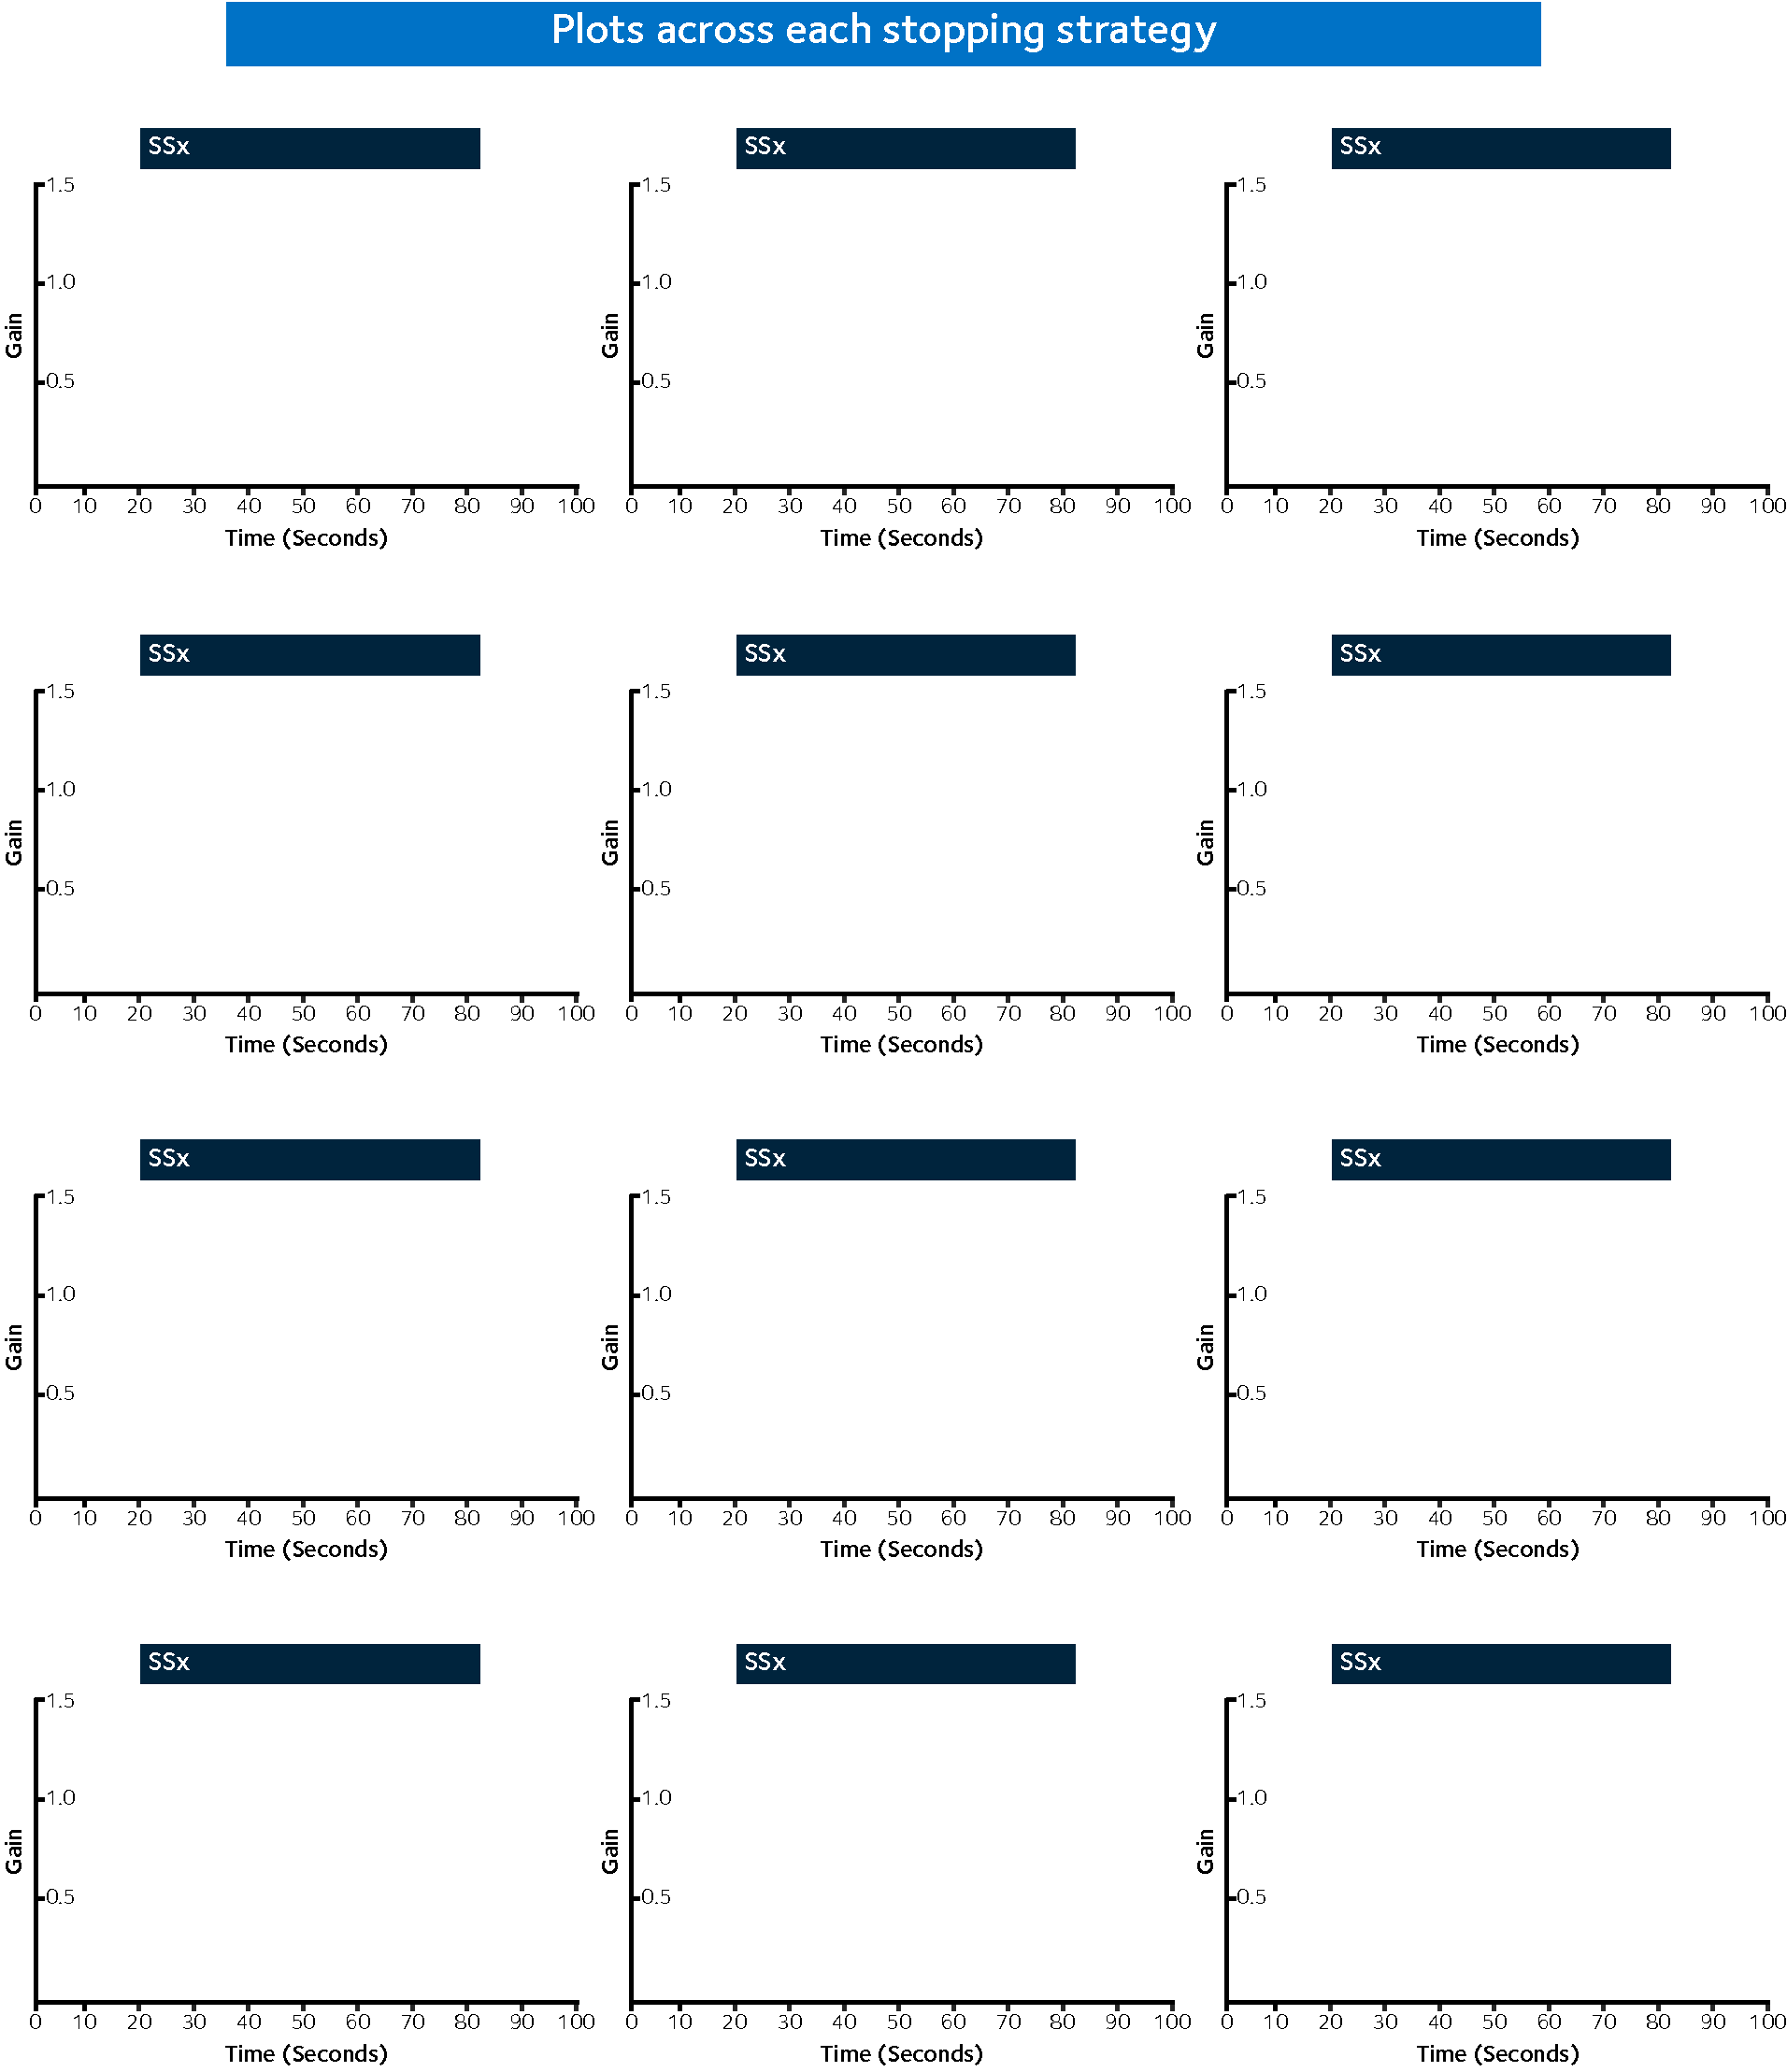
\includegraphics{figures/ch7-perf_plots_t0.pdf}}
    \caption[Blah]{Performance plots, T0}
    \label{fig:ch7_sim_perf_plots_t0}
\end{figure}

\begin{figure}[t!]
    \centering
    \resizebox{1\hsize}{!}{
    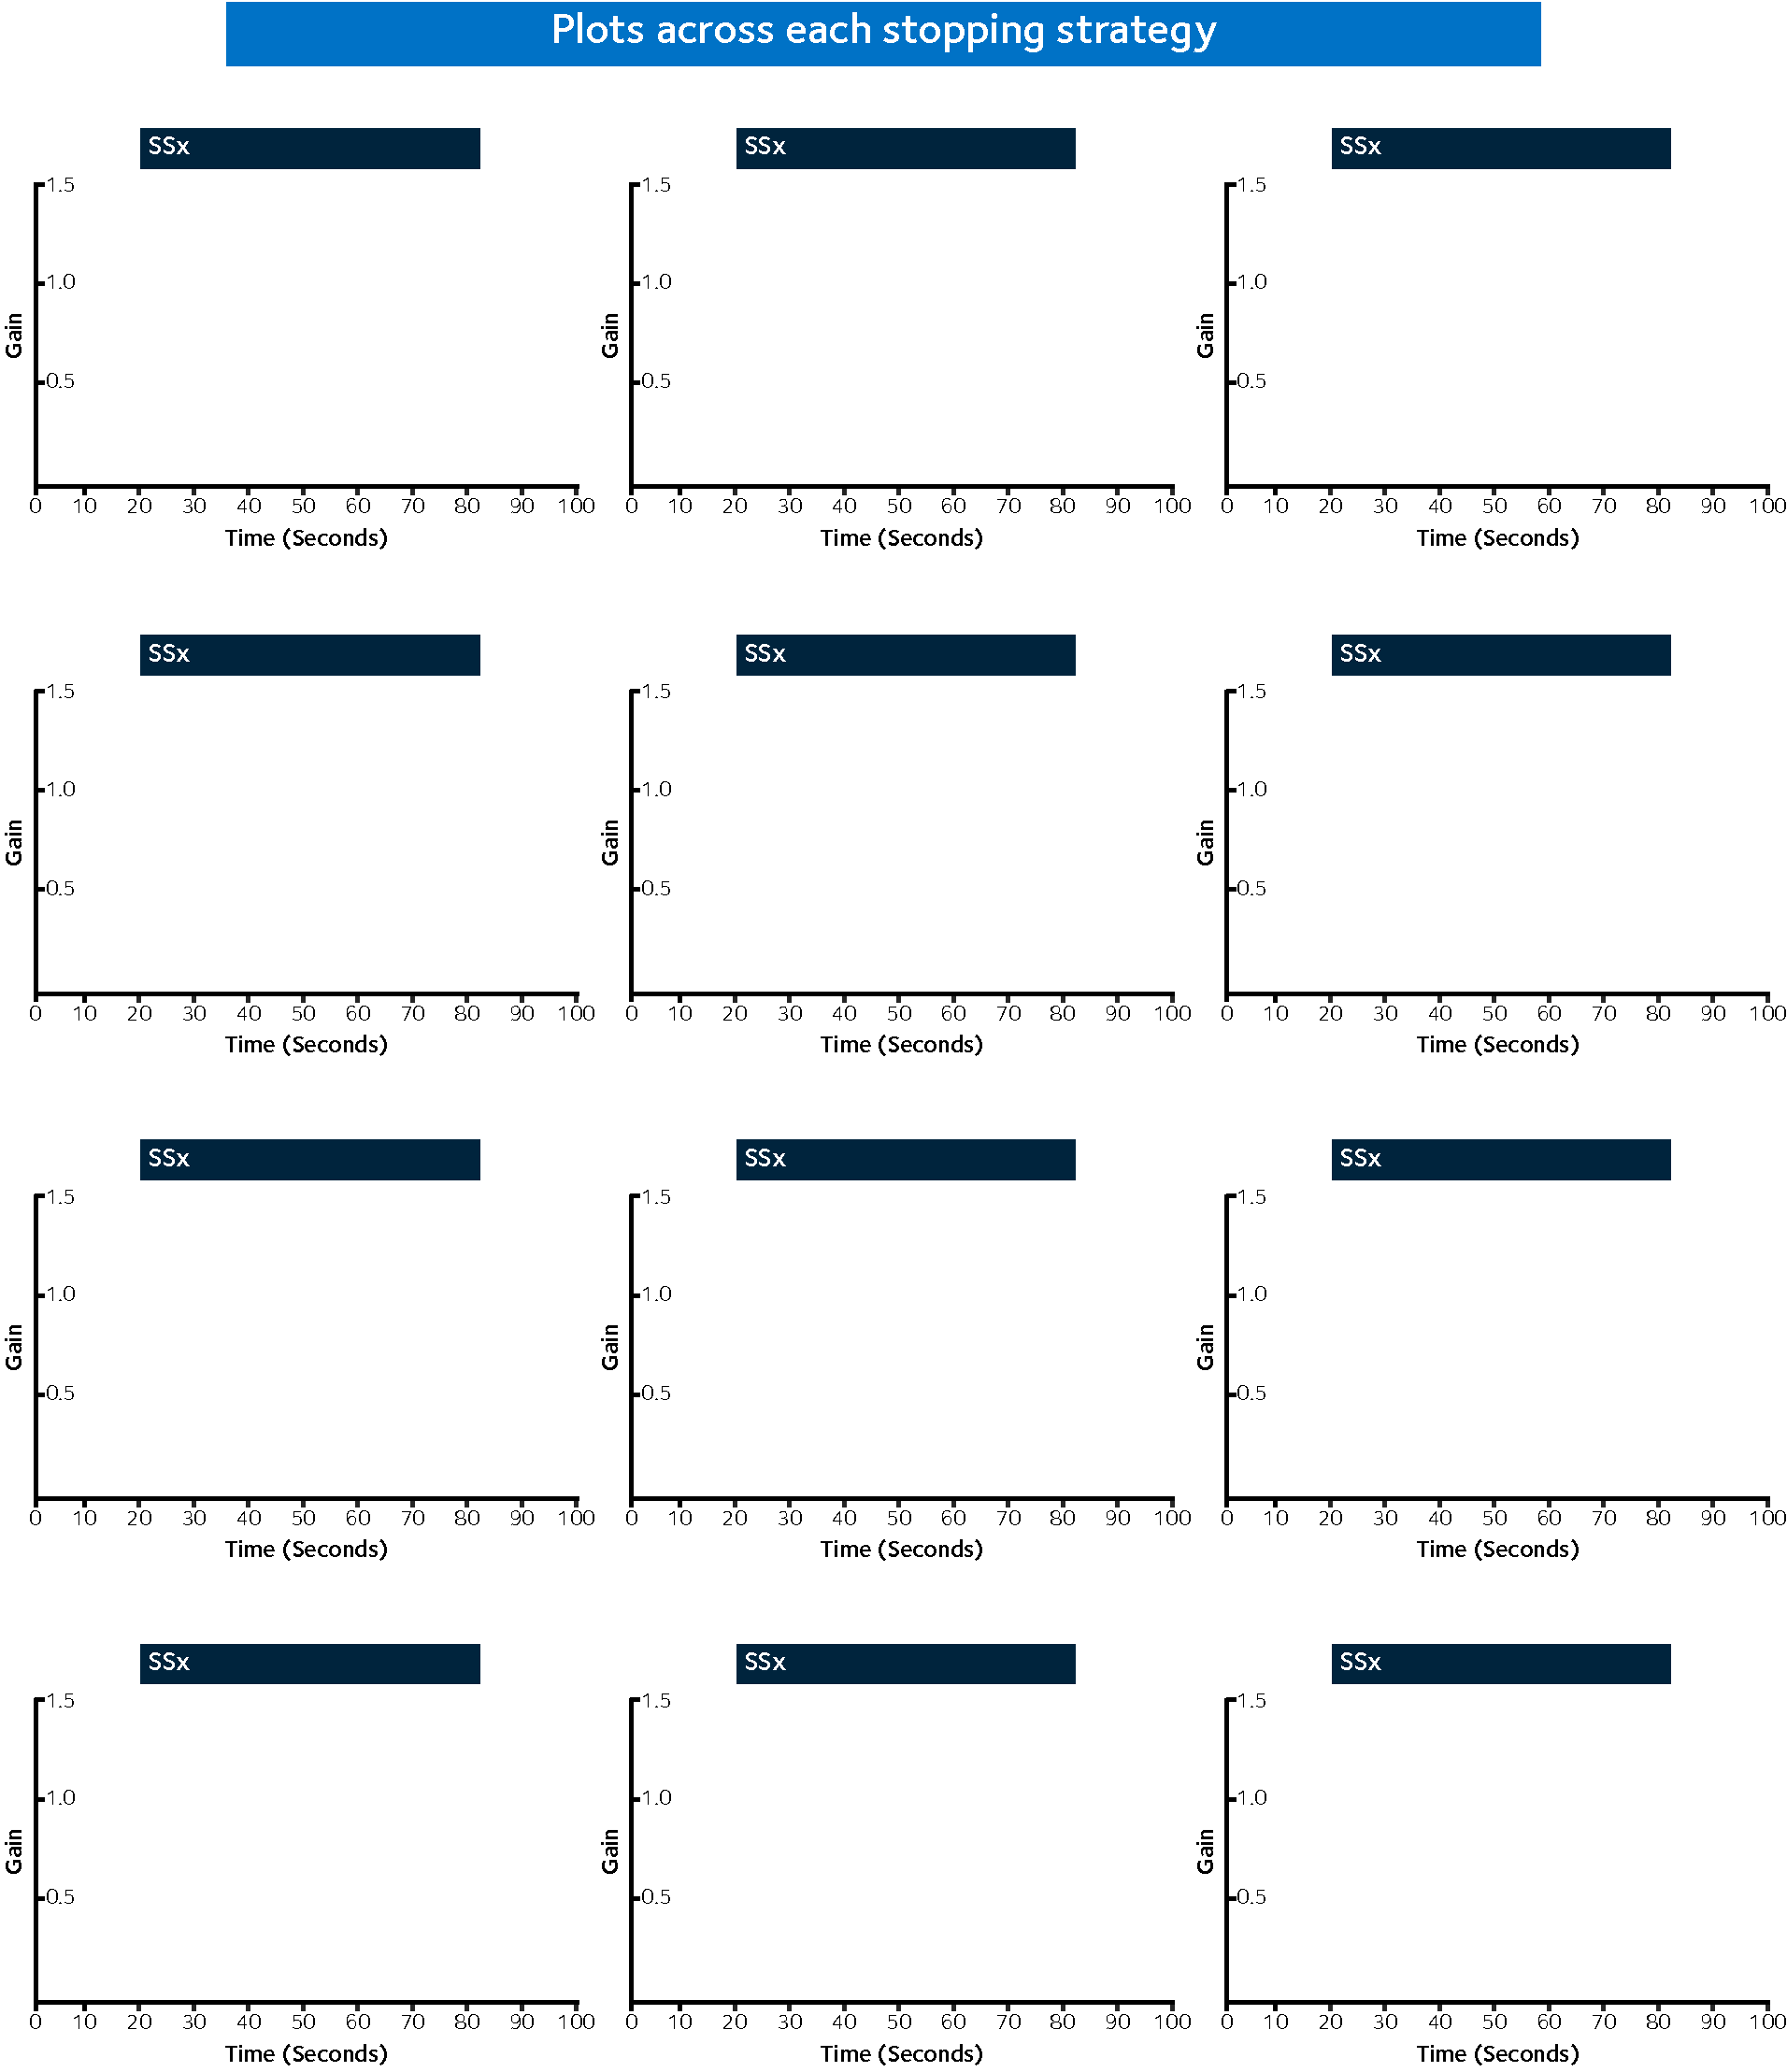
\includegraphics{figures/ch7-perf_plots_t0.pdf}}
    \caption[Blah]{Performance plots, T1}
    \label{fig:ch7_sim_perf_plots_t1}
\end{figure}

\begin{figure}[t!]
    \centering
    \resizebox{1\hsize}{!}{
    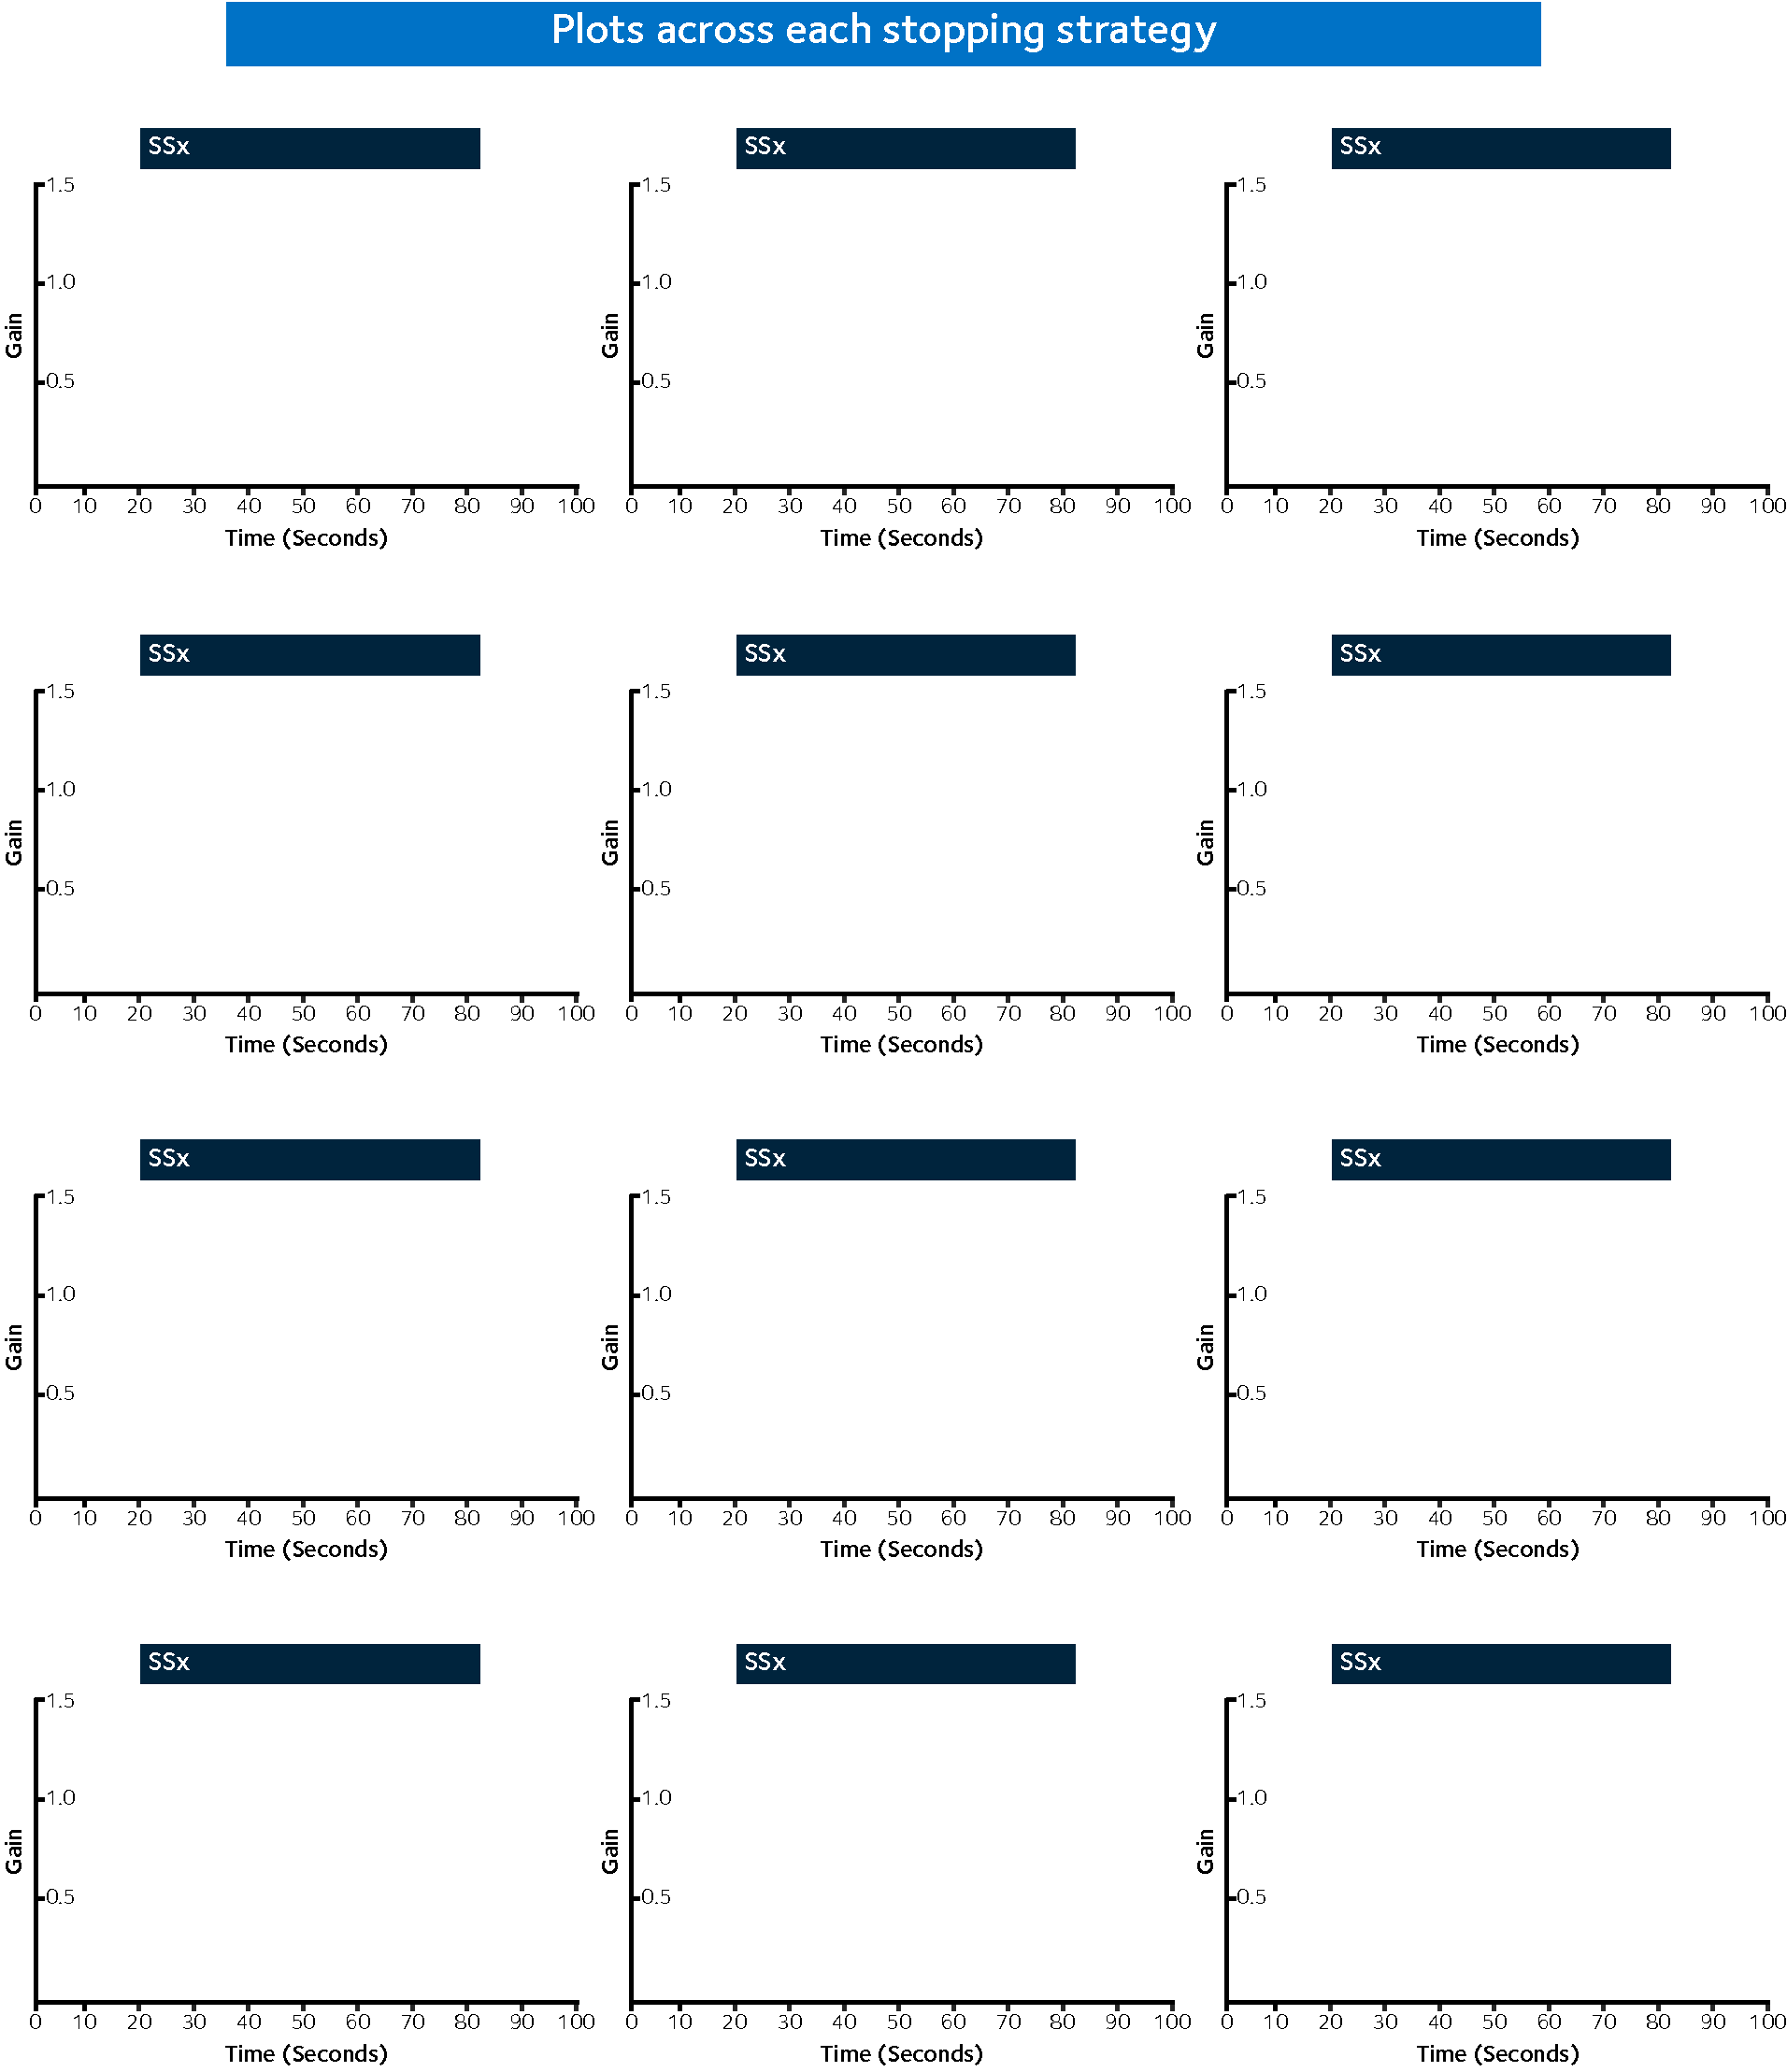
\includegraphics{figures/ch7-perf_plots_t0.pdf}}
    \caption[Blah]{Performance plots, T2}
    \label{fig:ch7_sim_perf_plots_t2}
\end{figure}

\begin{figure}[t!]
    \centering
    \resizebox{1\hsize}{!}{
    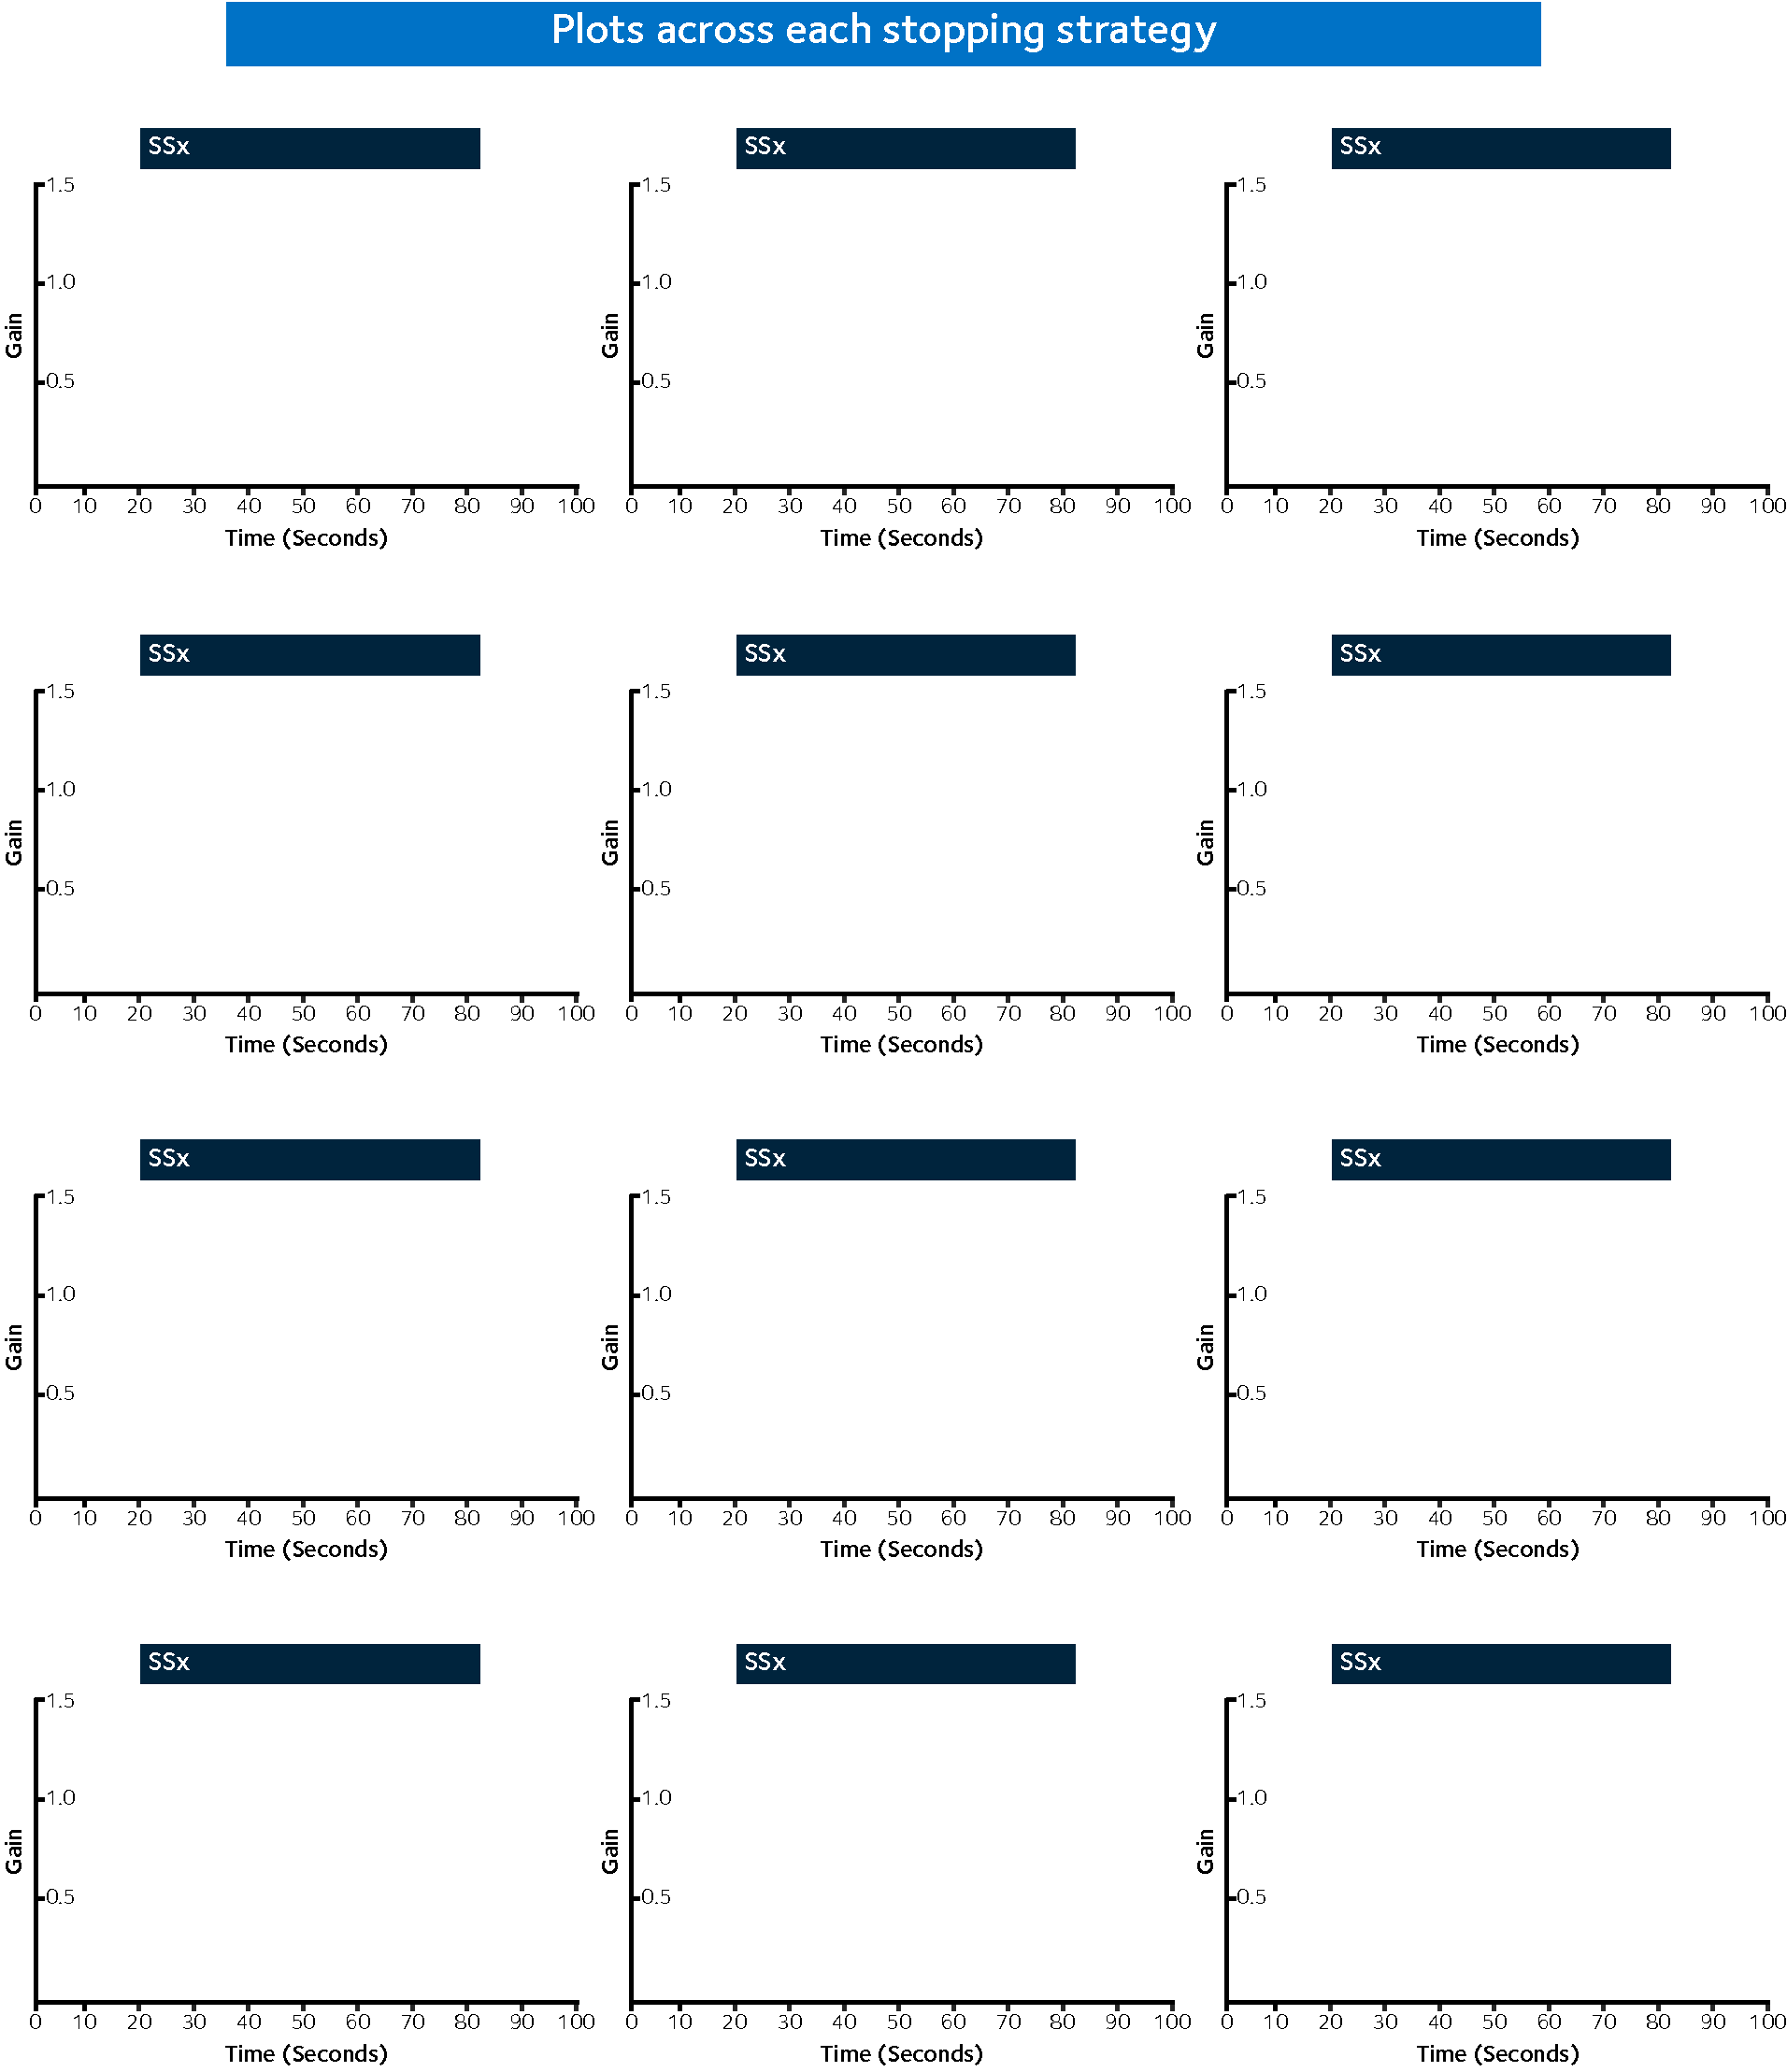
\includegraphics{figures/ch7-perf_plots_t0.pdf}}
    \caption[Blah]{Performance plots, T4}
    \label{fig:ch7_sim_perf_plots_t4}
\end{figure}

\begin{itemize}
    
    \item{First of all, how does the querying strategy perform? Take queries from all three strategies (QS1, QS3, QS13), and show that there's a sufficient variance between them. Show that QS1 produces poor queries on average, and QS3 produces better queries on average. Report the mean P@10 over a bunch of queries issued.}
    
    \item{PERFORMANCE}
    
    \item{Produce a grid of plots, 2x5 or something, that has one stopping strategy per plot. This is because some stopping strategies have two parameters, so you need to show what's going on as you vary the parameters. This needs to be repeated for each of the four interfaces. So four pages of plots?}
    
    \item{Each plot should have the upper bound, perfect decision maker line inserted, too.}
    
    \item{Produce a table, illustrating the highest levels of CG attained for each strategy, at what D/Q, and at what threshold(s). This must be done over each interface. This table, and the plots above, should be enough for one to be able to show what stopping strategies do best under what interface. Add some narrative, explaining each plot.}
    
    \item{COMPARISONS}
    
    \item{MSE plots, similar to above across each of the different stopping strategies and interfaces.}
    
    \item{Table(s) illustrating the lowest MSE for each SS. Include also the levels of CG that were attained by the searchers. Perhaps bring in the actual RW values, too, as per ECIR 2018.}
    
\end{itemize}

\subsubsection{Comparisons}

\subsubsection{Discussion}

\section{Chapter Summary}